\chapter{ISR Inversion}
\label{chapter:inversion}
\thispagestyle{myheadings}

% set this to the location of the figures for this chapter. it may
% also want to be ../Figures/2_Body/ or something. make sure that
% it has a trailing directory separator (i.e., '/')!
\graphicspath{{5_Inversions/Figures/}}

%%%%%%%%%%%%%%%%%%%%%%%%%%%%%%%%%%%%%%%%%%%%%%%%%%%%%%%%%%%%%%%%%%%%%%%%%
This chapter describes methods developed to invert the ISR space-time ambiguity function and improve on current reconstruction schemes. The first section briefly restates the forward model that was explored in depth in the earlier chapters. The follow section describes different inversion methods that have been used in the past in ISR along a single beam, thus removing only the range ambiguity. This leads next to a novel method of removing the effects of the full space-time ambiguity function described in Chapter~\ref{chapter:stamb} by reconstructing the parameters along the frame of reference of the moving plasma. The last section will demonstrate the reconstruction algorithms using both simple examples where non-linear fitting is not needed and runs from SimISR to determine the utility of algorithms on recovering the true plasma parameters.

\section{Forward Model}

ISR systems measure the ionospheric plasma parameters by estimating second order statistics from electromagnetic waves scattered from fluctuations of the electron density and fitting plasma parameters to these statistics. The second order statistics of the reflected waves, the ACF or power spectra, are related to the intrinsic plasma parameters through a physics based model, see Section~\ref{sec:incohscat}, and for greater detail Appendix~\ref{appendix1} for the specifics of this model. The full forward model of intrinsic ionospheric plasma parameters to measured parameters from ISR is represented in the diagram seen in Figure \ref{fig:flow1}. The measurement process starts with a set of plasma parameters distributed in time and space. Each set of plasma parameters is then transformed to a set of ACFs using the operator represented by $g()$. The space time ambiguity function $L$, acts as a blurring operator one might see in a camera or numerous other types of sensors. The estimates are then fit and estimates of the plasma parameters $\widehat{\boldsymbol{\theta}}$, are created. Often times these parameters are interpolated or projected back to the original Cartesian coordinate system, as the radar samples in a spherical coordinate space. This is in a way applying the adjoint operator $L^*$ to the fitted plasma parameters so researchers can compare to other sensors.

\begin{figure}[!ht]
\centering
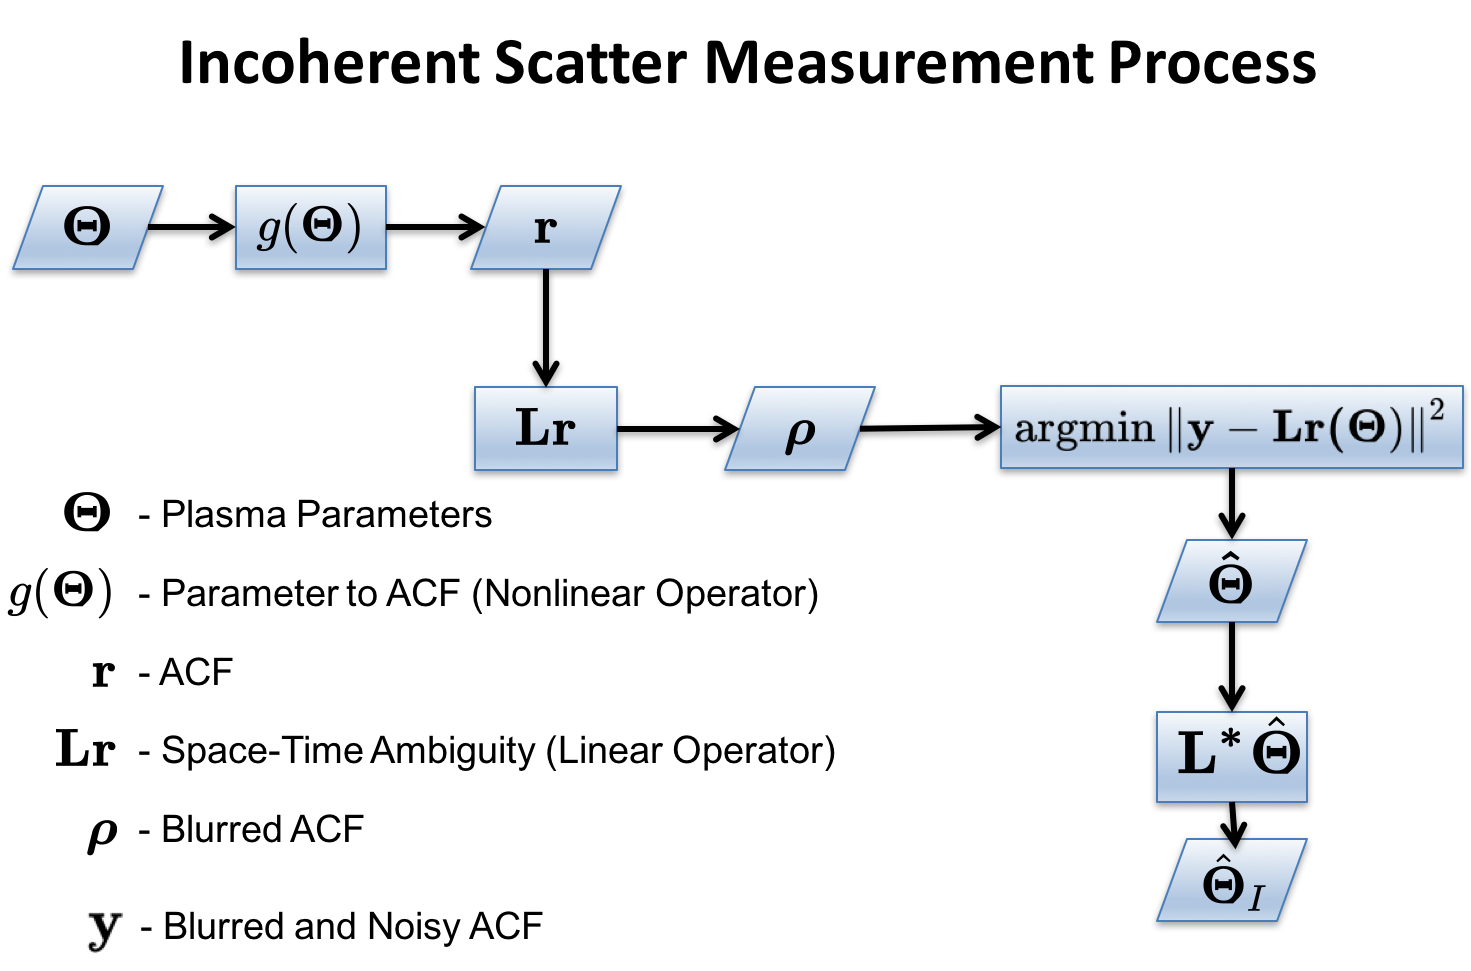
\includegraphics[width=.8\textwidth]{ladj}
\caption{ISR measurement formation process.}
\label{fig:flow1}
\end{figure}

This process shown in Figure \ref{fig:flow1} can be broken up into multiple parts. The linear portion of this, where the space-time ambiguity function $L$ is applied to the intrinsic ACFs in the ionosphere $R$, and creates measurements of the ACFs $\rho$, was detailed in Chapter~\ref{chapter:stamb}. Equation~\ref{eqn:sptamb}, restated in Equation~\ref{eqn:sptamb:inv}, shows this process as a Fredholm integral equation:
\begin{equation}
\label{eqn:sptamb:inv}
	\rho(\tau_s,\mathbf{r}_s,t_s) =\int L(\tau_s,\mathbf{r}_s,t_s,\tau,\mathbf{r},t)R(\tau,\mathbf{r},t)dVdtd\tau.
\end{equation}
Not stated in Equation~\ref{eqn:sptamb:inv} is the randomness within the measurement process. One way to model this is to take advantage of the fact that to order to estimate the ACFs a large number of pulses are averaged in ISR and using the central limit theorem, one can argue that the estimated ACFs become Normally distributed random variables \citep{papoulis2002}. The radar data can be modeled as follows $ y_s\sim \mathcal{CN}(\rho,\mathbf{C})$, where $\mathbf{C}$ is the covariance matrix of the ACFs,

\begin{equation}
\label{eqn:procsignal}
 y_s(\tau_s,\mathbf{r}_s,t_s) = \rho(\tau_s,\mathbf{r}_s,t_s) + w(\tau_s,\mathbf{r}_s,t_s),
\end{equation}

\noindent where $w(\tau_s,\mathbf{r}_s,t_s)$ is the zero mean random noise process of the ACFs with a correlation structure dictated by $\mathbf{C}$. 


As with nearly all practical inverse problems, it is necessary to carry on the inversion in a discrete space, so the algorithms be performed by digital computers. For this case the variable $y_s$ will be sampled set  in a vector format where each discrete point in lag (length $N_l$), time (length $N_t$) and space (length $N_s$) are vectorized along the index $i$. This will create a $N_lN_sN_t\times 1$ length vector 
\begin{equation}
\label{eqn:vec1}
\mathbf{y}=[y(\tau_0,\mathbf{r}_0,t_0), y(\tau_1,\mathbf{r}_1,t_1),..., y(\tau_{N_l N_s N_t -1}, \mathbf{r}_{N_l N_s N_t -1}, t_{N_l N_s N_t -1})]^T.
\end{equation}
The next step will be to discretize the input space, the intrinsic ACF in Cartesian coordinates, which will be represented by the vector $\mathbf{x}$, as $\mathbf{r}$ is already used for the spatial variable and $\mathbf{R}$ would imply a matrix variable. Like $\mathbf{y}$ each point in lag (length $N_v$), time (length $N_p$) and space (length $N_c$) are vectorized along the index $j$. The resulting $N_vN_pN_c\times 1$ length vector is the following,
\begin{equation}
\label{eqn:vecr}
\mathbf{x}=[R(\tau_0,\mathbf{r}_0,t_0), R(\tau_1,\mathbf{x}_1,t_1),..., R(\tau_{N_c N_p N_c -1}, \mathbf{r}_{N_v N_p N_c -1}, t_{N_v N_p N_c -1})]^T.
\end{equation}
The space-time ambiguity can be represented in a fully discretized form as the matrix $\mathbf{L}$. Substituting this into Equation \ref{eqn:procsignal} it becomes,
\begin{equation}
\label{eqn:procsignalvec}
 \mathbf{y} = \mathbf{L}\mathbf{x}+ \mathbf{w},
\end{equation}
\noindent where $\mathbf{x}$ is the intrinsic ACF in the Cartesian Coordinate space, and $\mathbf{w}$ is the vector of the noise process.

With the formulation in Equation~\ref{eqn:procsignalvec} schemes to reduce its impact of the Space-Time Ambiguity can be discussed.

%For standard ISR processing, the plasma parameters at each point in space and time individually. The cost function used is tries to reduce the error between the model ACF and the measured value in the least squares sense,
%
%\begin{equation}
%\label{eqn:lstsqrs}
%\widehat{\boldsymbol{\theta}_s} = \argmin\limits_{\boldsymbol{\theta}} \|y_s - g(\boldsymbol{\theta}_s) \|^2.
%\end{equation}
%
%\noindent The Levenberg-Marquart algorithm is often used to fit the plasma parameters to the final estimate ACFs \citep{levenberg1944,marquardt:1963,nikoukar2008}.

\section{Inversion Schemes}
\label{sec:isrlit}
The ambiguity function across range has been well studied and there have been a number of different methods proposed to reduce its impact on ISR measurements,
\citep{RDS:RDS3308,hysell2008,nikoukar2008,Virtanen:20082vx}. These methods fall into to two different categories of regularization. The first type, Full Profile Analysis \citep{RDS:RDS3308,hysell2008}, inverts the entire ISR process, including the non-linear step when moving between the parameter space and ACF space. This allows for parametric regularization which can include known physical constraints. The second type inverts only the range ambiguity as a linear operator and regularizes the estimated ACF. This is detailed in \citet{nikoukar2008} and \citet{Virtanen:20082vx}, and will be referred to data-based regularization.

The main trade-off between the two approaches is computational complexity versus accuracy of solution. Full Profile Analysis and other parametric regularization schemes require a large amount of computation to find a solution as the operator between the plasma parameters and ISR spectra is non-linear and thus many efficient and optimized techniques from linear inverse theory are not applicable. With data-based regularization techniques the computational requirements are significantly lowered as on is performing a linear inversion. Still this can lead to estimated ACFs that can not be created by the incoherent scattering operator.

%\section{Method Description}
%As discussed in Section \ref{sec:imgrec}, the main trade-off between the two approaches, parametric and data based reconstruction, is computational complexity versus accuracy of solution. Full profile analysis and other parametric regularization schemes require a large amount of computation to find a solution, as the operator between the plasma parameters and ISR spectra is non-linear and thus various techniques from linear inverse theory are not completely applicable. With data-based regularization techniques the computational requirements are significantly lowered as one is performing a linear inversion. Still this can lead to estimated ACFs that can not be created by the incoherent scattering operator.
%
%In order to reconstruct the field of plasma parameter values we treat the space-time ambiguity as a linear operator, acting on the true intrinsic ACF of the plasma and outputting noisy and blurred estimates, which are then fitted to plasma parameters. This allows for the use of inversion schemes from image processing. In this case, using $y$ for the estimate of the ACF, $\rho$ seen in equation, Equation~\ref{eqn:sptamb}, the objective function, with no regularization would be 
%
%\begin{equation}
%\label{eqn:lstsqrs:opt}
%\argmin\limits_{R} \| y_s(\tau_s,\mathbf{r}_s,t_s)- \int L(\tau_s,\mathbf{r}_s,t_s,\tau,\mathbf{r},t)R(\tau,\mathbf{r},t)dVdtd\tau \|^2.
%\end{equation}

%\section{Introduction}
%
%Incoherent scatter radar (ISR) measures plasma parameters by fitting plasma parameters to an estimate of the auto correlation function (ACF) from the inherent fluctuations in electron density in the ionosphere. In order to perform this estimate the radar has to create an average of ACF over time and space. This averaging acts as a linear operator over time and space for the estimated ACFs and creates an ambiguity for the measurements. The direct impact of the operator on the measurement of plasma parameters can be difficult to assess as the relationship between plasma parameters and the ACF is non-linear. 
%
%The development of the Advanced Modular Incoherent Scatter Radar (AMISR) systems, with its electronically-scannable antenna, have allowed for three dimensional reconstruction of plasma parameters. In order to analyze the performance of these systems the idea of the ambiguity function had to be extended to include the antenna beam pattern and the time dimension referred to as the space-time ambiguity function in  \citep{RDS:RDS20236}. 
%
%With the linearity assumption many ideas in linear inverse theory can be applied. There is a large amount of literature in this area, mainly in image processing and reconstruction \citep{Karl:2005jy}, and could be used to invert the operator and improve the resolution of the measurement. 
%
%This paper will cover the a method for inverting this space-time ambiguity function. In order to test this method we use synthetic data from the Simulation for ISR (SimISR), driven by a ionosphere plasma state parameters from a multi-fluid ionosphere model \citep{semeter:plasmatransport2012}. The following sections of this paper are as follows. Section \ref{sec:isramb} describes the ISR image formation process in the language of inverse theory. Following this, Section \ref{sec:isrlit} details the use of inverse theory in single dish ISR systems to reconstruct altitude profiles. Section \ref{sec:isralg} describes our specific algorithm that has been developed and following in Section \ref{sec:results}, we show results of these reconstructions.

%\section{ISR Space-Time Ambiguity}
%\label{sec:isramb}
%The ISR processing can be represented in the diagram seen in Figure \ref{fig:flow1}. The image formation process starts with a set of plasma parameters distributed in time and space. Each set of plasma parameters is then transformed to a set of ACFs using the operator represented by $g()$. The space time ambiguity function $L$ acts as a blurring operator one might see in a camera or numerous other types of sensors. The estimates are then fit and estimates of the plasma parameters, $\widehat{\boldsymbol{\theta}}$, are created. Often times these parameters are interpolated or projected back to the original Cartesian coordinate system, this is in a way applying the adjoint operator $L^*$ to the fitted plasma parameters to create a 
%
%
%The space-time ambiguity, $L(\tau_s,\mathbf{r}_s,t_s,\tau,\mathbf{r},t)$, can be treated as the kernel of a Fredholm integral equation of the first kind operating on the ACF, $R(\tau,\mathbf{r},t)$, which can change over space, $\mathbf{r}$, and time $t$, i.e.,
%
% \begin{equation}
%  \label{eqn:staf}
%  \rho(\tau_s,\mathbf{r}_s,t_s) =\int L(\tau_s,\mathbf{r}_s,t_s,\tau,\mathbf{r},t)R(\tau,\mathbf{r},t)dVdtd\tau,
%\end{equation}

%\noindent where the subscript $s$ represents the same variable but now discretely sampled by the radar. 
%
%The kernel is a separable function when the spatial coordinates are spherical, centered at the radar, where ($r,\theta,\phi)$ represent, range, azimuth and elevation respectively. This the changes Equation \ref{eqn:staf} as follows,
%
%\begin{equation}
%\label{eqn:stafbrok}
%\rho(\tau_s,\mathbf{r}_s,t_s)= \int G(t_s,t)F(\theta_s,\phi_s,\theta,\phi)W(\tau_s,r_s,\tau,r) R(\tau,\mathbf{r},t) dVdt d\tau,
%\end{equation}
%
%\noindent where $G(t_s,t)$ is the kernel for the time dimension, $F(\theta_s,\phi_s,\theta,\phi)$ is radar beam shape which acts as a kernel in azimuth and elevation, and $W(\tau_s,r_s,\tau,r) $ which is the range ambiguity function which acts as a kernel along range $r$ and lag $\tau$. The derivation of this operator can be seen in \citep{RDS:RDS20236}.
%
%
%\begin{figure}[!ht]
%    \centering
%    \begin{subfigure}[b]{0.47\textwidth}
%        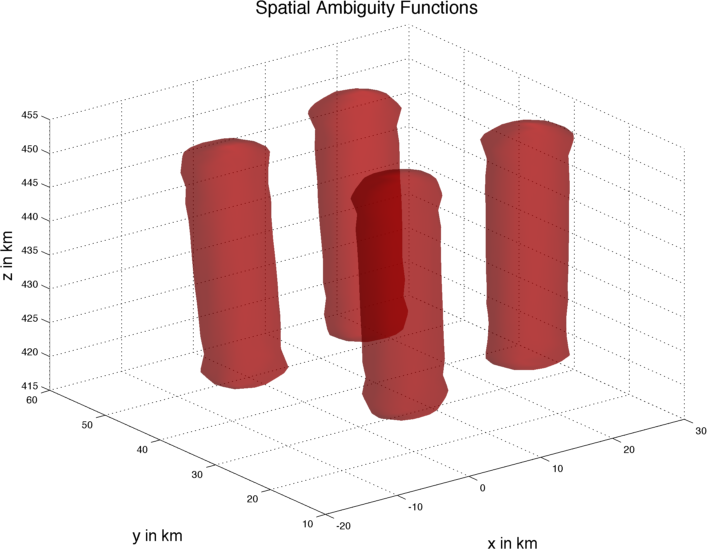
\includegraphics[width=\textwidth]{spaceamb}
%        \caption{Stationary.}
%        \label{fig:Amb1}
%    \end{subfigure}
%    ~ %add desired spacing between images, e. g. ~, \quad, \qquad, \hfill etc. 
%      %(or a blank line to force the subfigure onto a new line)
%    \begin{subfigure}[b]{0.47\textwidth}
%        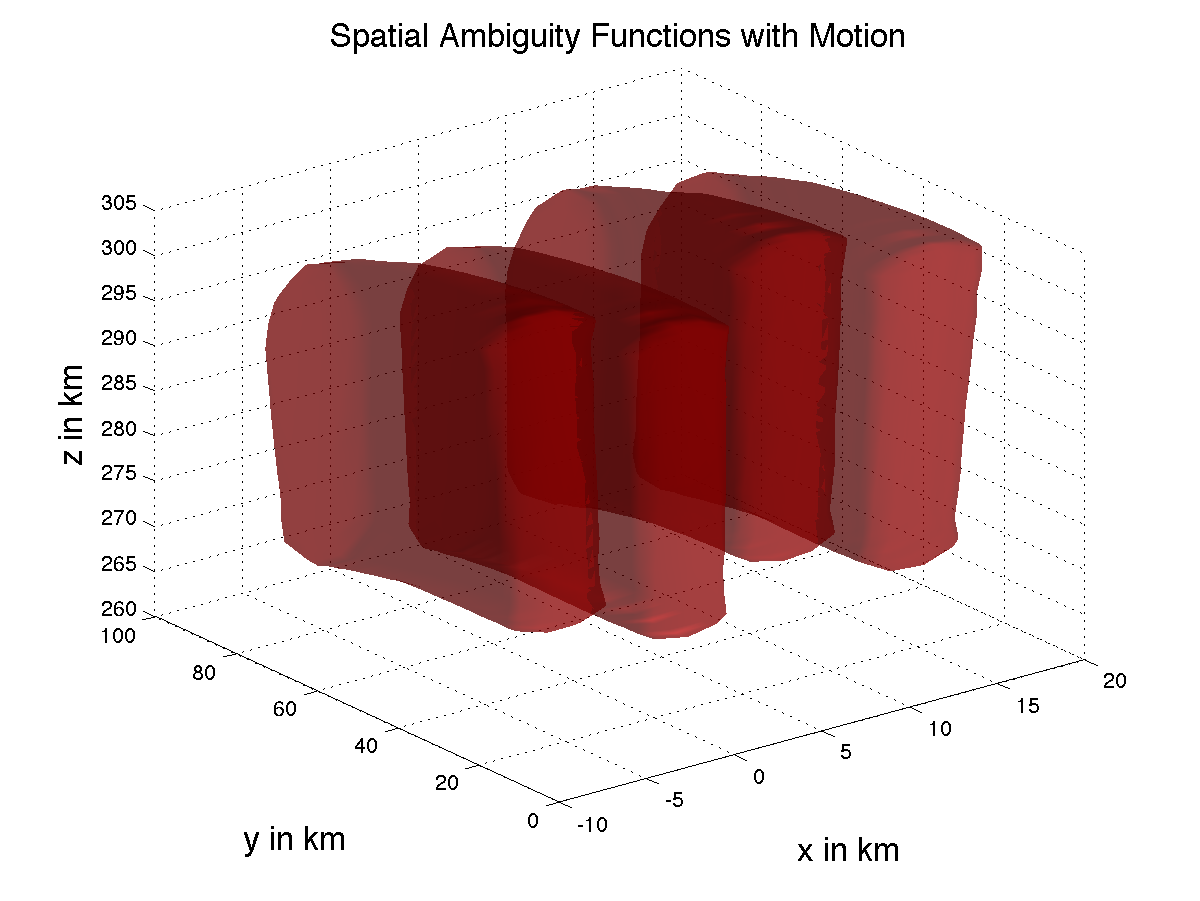
\includegraphics[width=\textwidth]{spaceambmoving}
%        \caption{With 500 m/s drift.}
%        \label{fig:Ambmoving}
%    \end{subfigure}
%
%    \caption{Space time ambiguity function.}\label{fig:Ambboth}
%\end{figure}
%
%The ambiguity found in Cartesian space in Figure \ref{fig:Amb1}. The ambiguity is interesting in a number of ways. First it is non-isotropic in space so it is important to know the orientation of the beam and its shape otherwise this may cause errors in any inversion scheme. Another aspect is that the blurring in incurs is shift variant in space, so it is not a convolution and thus any methods specific for those problems will not apply. Lastly, like in cameras if there is motion in the plasma during the integration period then a motion blur will also be added. This will change the ambiguity in the rest frame of the plasma to be closer to what is seen in Figure \ref{fig:Ambmoving}.

%In order to estimate the ACFs a large number of pulses need to be integrated. Using the central limit theorem on can argue that the estimated ACFs become Normally distributed random variable \citep{papoulis2002}. The radar data can be modeled as follows $ y_s\sim \mathcal{CN}(\rho,\mathbf{C})$, where $\mathbf{C}$ is the covariance matrix of the ACFs, or even,
%
%\begin{equation}
%\label{eqn:procsignal}
% y_s(\tau_s,\mathbf{r}_s,t_s) = \rho(\tau_s,\mathbf{r}_s,t_s) + w(\tau_s,\mathbf{r}_s,t_s),
%\end{equation}
%
%\noindent where $w(\tau_s,\mathbf{r}_s,t_s)$ is the ACF of the noise process. 
%
%For standard ISR processing, the plasma parameters at each point in space and time individually. The cost function used is tries to reduce the error between the model ACF and the measured value in the least squares sense,
%
%\begin{equation}
%\label{eqn:lstsqrs}
%\widehat{\boldsymbol{\theta}_s} = \argmin\limits_{\boldsymbol{\theta}} \|y_s - g(\boldsymbol{\theta}_s) \|^2.
%\end{equation}
%
%\noindent The Levenberg-Marquart algorithm is often used to fit the plasma parameters to the final estimate ACFs \citep{levenberg1944,marquardt:1963,nikoukar2008}.
%%%%%%%%%%%%%%%%%%%%%%%%%%%%%%%%%%%%%%%%%%%%%%%%%%%%%%%%%%%%%%%%%%%%%%%


For the case of parametric based reconstruction schemes, such as full profile analysis, the goal is to reconstruct the full set of plasma parameters at each point in time and space, represented as the matrix $\boldsymbol{\Theta}$. The cost function for this is the following, 

\begin{equation}
\label{eqn:lstsqrsvecpb}
\widehat{\boldsymbol{\Theta}} = \argmin\limits_{\boldsymbol{\Theta}} \|\mathbf{y} -\mathbf{L}\mathbf{ g}(\boldsymbol{\Theta}) \|^2 + \boldsymbol{\alpha}\cdotp\mathbf{f}(\boldsymbol{\Theta}),
\end{equation}

\noindent where $\mathbf{f}(\boldsymbol{\Theta})$ is a vector of constraints functionals based on the plasma parameters, $\boldsymbol{\alpha}$ is a vector that holds the different weightings for these constraints.

With data based reconstruction, the inversion is based on removing the effect of the space time ambiguity function on the ACFs and then subsequently fitting the plasma parameters. The cost function, similar to Equation \ref{eqn:lstsqrsvecpb}, is the following

\begin{equation}
\label{eqn:lstsqrsvecdb}
\widehat{\mathbf{x}} = \argmin\limits_{\mathbf{x}} \|\mathbf{y} -\mathbf{Lx} \|^2 + \boldsymbol{\gamma}\cdotp\mathbf{f}(\mathbf{x}),
\end{equation}

\noindent where $\mathbf{f}(\mathbf{x})$ is a vector of constraint functionals based on the ACFs, $\boldsymbol{\gamma}$ is a vector that holds the different weightings for these constraints. The ACFs are then fit to plasma parameters at each point in space and time using a non-linear least squares algorithm as in standard processing schemes, see Section~\ref{section:isrproc}.

%The best way to compare and contrast the two formats is to first pose the problem in a vector format, first each time and spatial vector are rasterized along the index $i$. Next the discrete estimate of each ACF can be placed in an $L$ length single vector for each space-time index $i$,
%
%\begin{equation}
%\label{eqn:vec1}
%\mathbf{y}_i=[y(\tau_0,\mathbf{r}_i,t_i), y(\tau_1,\mathbf{r}_i,t_i),..., y(\tau_{L-1},\mathbf{r}_i,t_i)].
%\end{equation}
%
%\noindent This vector $y_i$ can be come the $i^{th}$ row in the matrix $\mathbf{Y}$,
%
%\begin{equation}
%\label{eqn:matall}
%\mathbf{Y}=[\mathbf{y}_0^T,\mathbf{y}_1^T, ..., \mathbf{y}_{NM}^T]^T
%\end{equation}
%
%\noindent where $N$ is number of locations that were sampled by the radar and $M$ is the number of times. With this representation Equation \ref{eqn:procsignal} becomes
%
%\begin{equation}
%\label{eqn:matsigproc}
%\mathbf{Y} = \boldsymbol{\rho} + \mathbf{W},
%\end{equation}
%
%\noindent where $\mathbf{W}$ is the $NM\times L$ noise matrix. 




%There may be some way in between. In \citep{Oktem:2014ju} data from spectral imagers are inverted with a nonlinear step involved. This type of technique only takes into account data from pixels that are near to the point of interest. This could be useful in ISR due to the fact that contributions from far away points is rather small due to the beam pattern. 
%
%Another aspect that needs to be explored is the possibility of using an iterative technique that where the ACFs are estimated and then fit to plasma parameters iteratively. This could yield a solution that would reduce computational complexity but improve the accuracy of the solutions.

\section{Reconstruction in the Frame of Moving Plasma}
\label{sec:isralg}
Due to the size of the problem the inversion methods focused on in this work are data based regularization cost functions of the type seen in Equation \ref{eqn:lstsqrsvecdb}. The space time ambiguity matrix $\mathbf{L}$ has a block matrix form with the sub-matrix $\mathbf{K}$ representing the spatial ambiguity. This block structure can be expressed as

\begin{equation}
\label{eqn:kmat}
\mathbf{L}= \begin{bmatrix}\mathbf{K}&\cdots&\mathbf{K}&\mathbf{0}&\cdots&&\mathbf{0}\\
\mathbf{0}&\cdots&&\mathbf{K}&\cdots&\mathbf{K}&\mathbf{0}\\
\vdots&&&\ddots&&&\vdots\\
\mathbf{0}&&&\cdots&\mathbf{K}&\cdots&\mathbf{K}
\end{bmatrix},
\end{equation}

\noindent where $\mathbf{0}$ is a matrix of zeros the same size as $\mathbf{K}$. This representation has some advantages as the inverse problem can be broken up into smaller pieces. However, this still leads to rather large matrices to invert because the number of rows grow with the number of time frames along the input are integrated. 

Another representation that can drop the calculations down further entails adjusting the spatial ambiguity to take into account the velocity of the plasma. Using a Galilean Transform like in \citet{RDS:RDS20236}, the set of $\mathbf{K}$ matrices for each time integration can become a single matrix $\mathbf{A}_{m,n}$. This form is shown as the following:

\begin{equation}
\label{eqn:amat}
\mathbf{L}= \begin{bmatrix}
\mathbf{A}_{0,0}&\mathbf{0}&\cdots&\mathbf{0}\\
 \mathbf{0}&\mathbf{A}_{1,1}&\mathbf{0}&\\
 \vdots&&\ddots&\vdots\\
 \mathbf{0}&\cdots&&\mathbf{A}_{N_T-1,N_T-1}
\end{bmatrix}.
\end{equation}

\noindent This new version of $\mathbf{L}$ will lead to ACFs in the moving frame of reference. The approach assumes a stationary morphology of the plasma parameters. This assumption may be physically justified for certain high latitude scenarios, where the regional ionosphere probed by an ISR could be described as a structured field (structured by particle precipitation or plasma patch transport) translating according to a regionally uniform convective flow pattern~\citep{Tsunoda:1988ul}.

In order to speed up the reconstruction, each individual lag and time frame of the ACF separately are handled separately. The time frame is obvious from the structure of the new $\mathbf{L}$ seen in Equation~\ref{eqn:amat}. The ability to separate each lag is assuming that the receiver filter bandwidth is sufficient that it does not impact the shape of the IS spectrum. These assumptions lead to the following cost function

\begin{equation}
\label{eqn:lstsqrsvecdblag}
\widehat{\mathbf{x}_{m,l}} = \argmin\limits_{\mathbf{x}_{m,l}} \|\mathbf{y}_{m,l} -\mathbf{L}_{m,l}\mathbf{x}_{m,l} \|^2 + \boldsymbol{\gamma}\cdotp\mathbf{f}(\mathbf{x}_{m,l}),
\end{equation}
\noindent where the indexes $m$ and $l$ represent time and lag respectively. In order to solve the cost functions the package CVXPY is used \citep{cvxpy}.

For this study, three specific cost functions are used. The first is a constraint on the $l^2$-norm of the solution $\mathbf{x}_{m,l}$, which can be represented as the following cost function,
\begin{equation}
\label{eqn:tikpow}
\widehat{\mathbf{x}_{m,l}} = \argmin\limits_{\mathbf{x}_{m,l}} \|\mathbf{y}_{m,l} -\mathbf{L}_{m,l}\mathbf{x}_{m,l} \|^2 +\gamma_{m,l} \|\mathbf{x}_{m,l}\|^2.
\end{equation}

\noindent This type of regularization is generally referred to as Tikhonov Regularization \citep{Karl:2005jy}.

The next type of constraint is also a $l^2$-norm constraint on the solution, i.e. Tikhonov Regularization, except that it operates on $\mathbf{D}\mathbf{x}_{m,l}$, a numerical approximation to the spatial gradient of $\mathbf{x}_{m,l}$. The cost function is the following,

\begin{equation}
\label{eqn:tikD}
\widehat{\mathbf{x}_{m,l}} = \argmin\limits_{\mathbf{x}_{m,l}} \|\mathbf{y}_{m,l} -\mathbf{L}_{m,l}\mathbf{x}_{m,l} \|^2 + \gamma_{m,l} \|\mathbf{D}\mathbf{x}_{m,l}\|^2.
\end{equation}

\noindent The last constraint is similar to Equation \ref{eqn:tikpow} but instead uses an $l^1$-norm,
\begin{equation}
\label{eqn:tv}
\widehat{\mathbf{x}_{m,l}} = \argmin\limits_{\mathbf{x}_{m,l}} \|\mathbf{y}_{m,l} -\mathbf{L}_{m,l}\mathbf{x}_{m,l} \|^2 + \gamma_{m,l} \|\mathbf{D}\mathbf{x}_{m,l}\|.
\end{equation} 

\noindent This constraint is generally referred to as \textit{total variations} regularization and has been used in image processing \citep{Rudin:1992kn}

\section{Results}
\label{sec:results}
This section presents two different examples of inversion algorithm performance. The first case shows how  the inversion methods work on reversing the linear process of the space time ambiguity function, which is equivalent to applying the reconstruction to the zeroth ACF lag. The second example employs data from SimISR, which was detailed in Chapter~\ref{chapter:stisrs}. This example will apply the reconstruction algorithms to ACFs and then apply the non-linear fitting to measure the plasma parameters.

For both cases the velocities of the features are assumed to be known. There have been schemes in the past that have reconstructed the plasma flow velocities using the Doppler shift in the ISR spectrum, such as in \citet{butler:imagingfregiondrifts}, which similarly lead to an assumption of stationarity of the plasma parameters in the rest frame of the moving plasma. The constraint parameters $\gamma_{m,l}$, were selected by searching a number of parameter values and taking the minimum mean squared error result. There are other methods of choosing this parameter such as L-curve analysis \citep{Karl:2005jy}. 

\subsection{Single Lag Example}

The first example shows the performance of the algorithm on data that has been created from the linear processing of the space-time ambiguity function, or essentially the reconstruction of the zeroth ACF lag. The data consists of a two dimensional phantom with a background chapman function and an enhancement moving through at 2.5 km/s. The enhancement is shaped as a bump function along the horizontal axis which peaks at three times the background. The input phantom at $t=0$ and $t=57$ can be seen in Figures \ref{fig:simpinputfast}a and \ref{fig:simpinputfast}b. The result of applying the operator can be seen in Figure \ref{fig:simpinputfast}c and shows the enhancement smeared out across the field of view.

\begin{figure}[!ht]
\centering
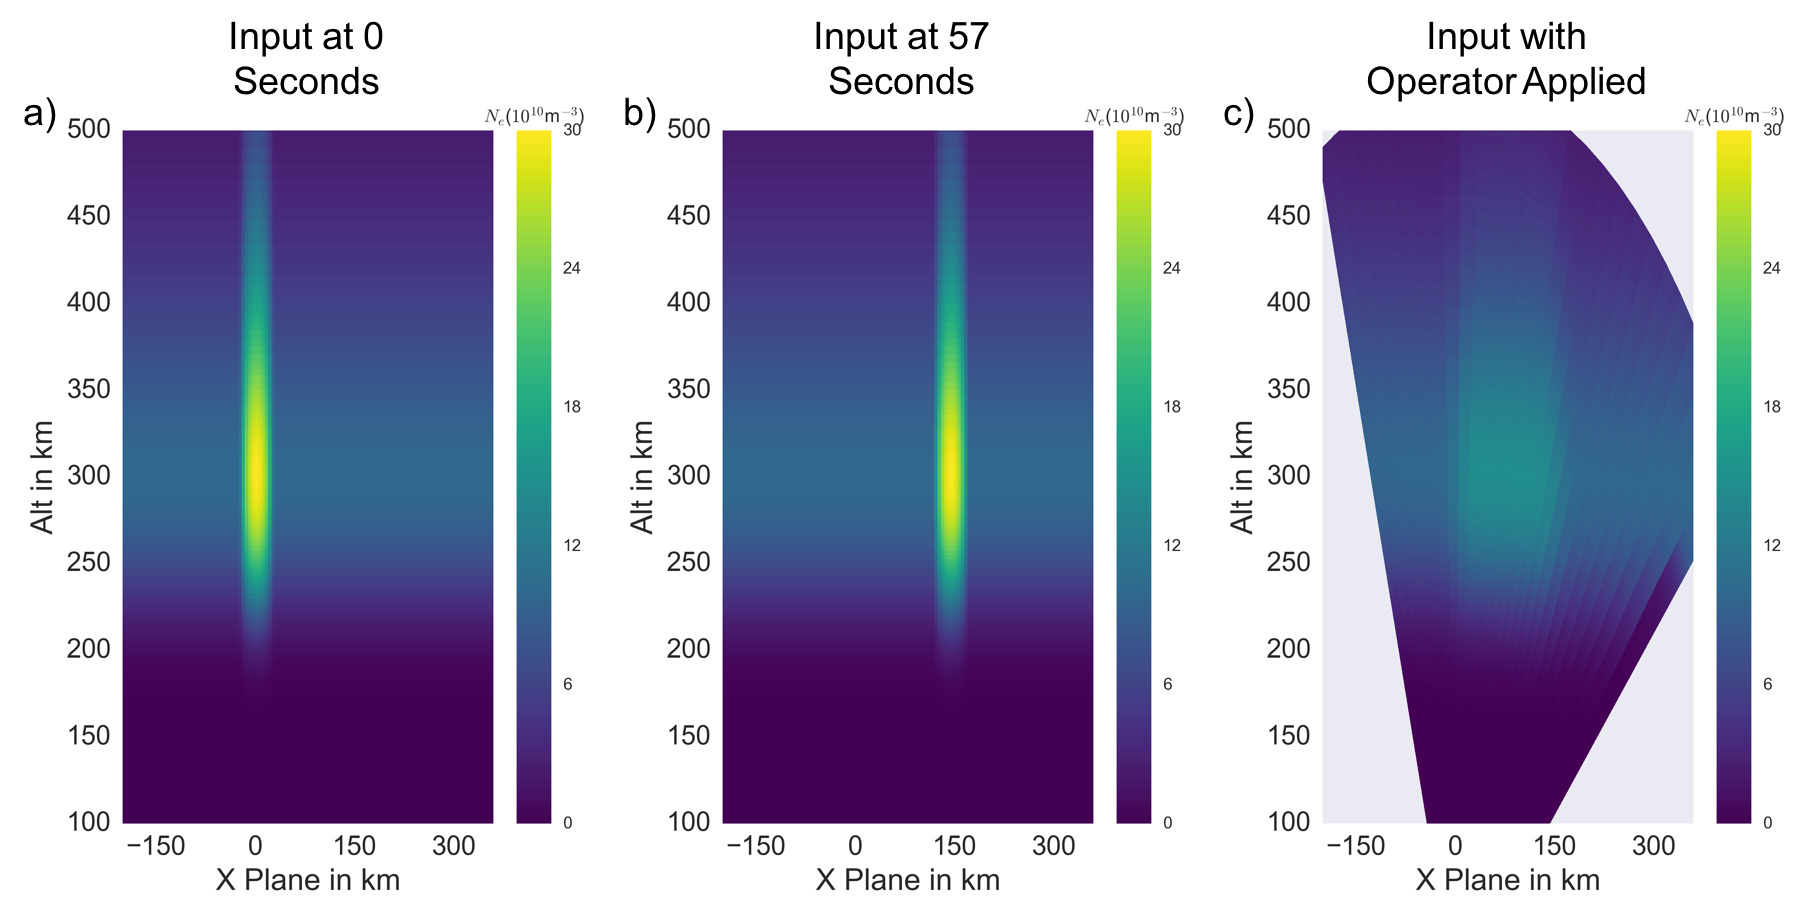
\includegraphics[width=6in]{Simpleinputfast}
\caption{a) The Input phantom at 0 seconds. b) The input phantom at 57 seconds. c) The average of the moving phantom with the ambiguity applied.}
\label{fig:simpinputfast}
\end{figure}

The results of the different algorithms can be seen in Figure \ref{fig:simpoutputfast}. Using a simple Tikhonov constraint on the energy of the function, the reconstruction, seen in Figure \ref{fig:simpoutputfast}a, shows a number of artifacts. The behavior of this algorithm is to reduce the power from areas that are not passed through the imaging process, and thus he results trace a beam pattern in the reconstruction. The reconstruction using an $l^2$-norm constraint on the derivative operator, seen in Figure \ref{fig:simpoutputfast}b, shows good correspondence with the input phantom although there is some carving out of the electron density near the enhancement. Lastly the reconstruction using a reconstruction using the $l^1$-norm constraint on the derivative operator, or \textit{total variations} is shown in Figure \ref{fig:simpoutputfast}c. This reconstruction has a ``blocky" appearance as is the common trait of these sorts of reconstructions due to the tendency of the $l^1$-norm constraint to return solutions that are sparse with respect to the constraint function, in this case the spatial gradient of the zeroth lag of the ACF. This can be expected for total variations as has been very popular in use of reconstructing high contrast images \citep{Karl:2005jy}. 

\begin{figure}[!ht]
\centering
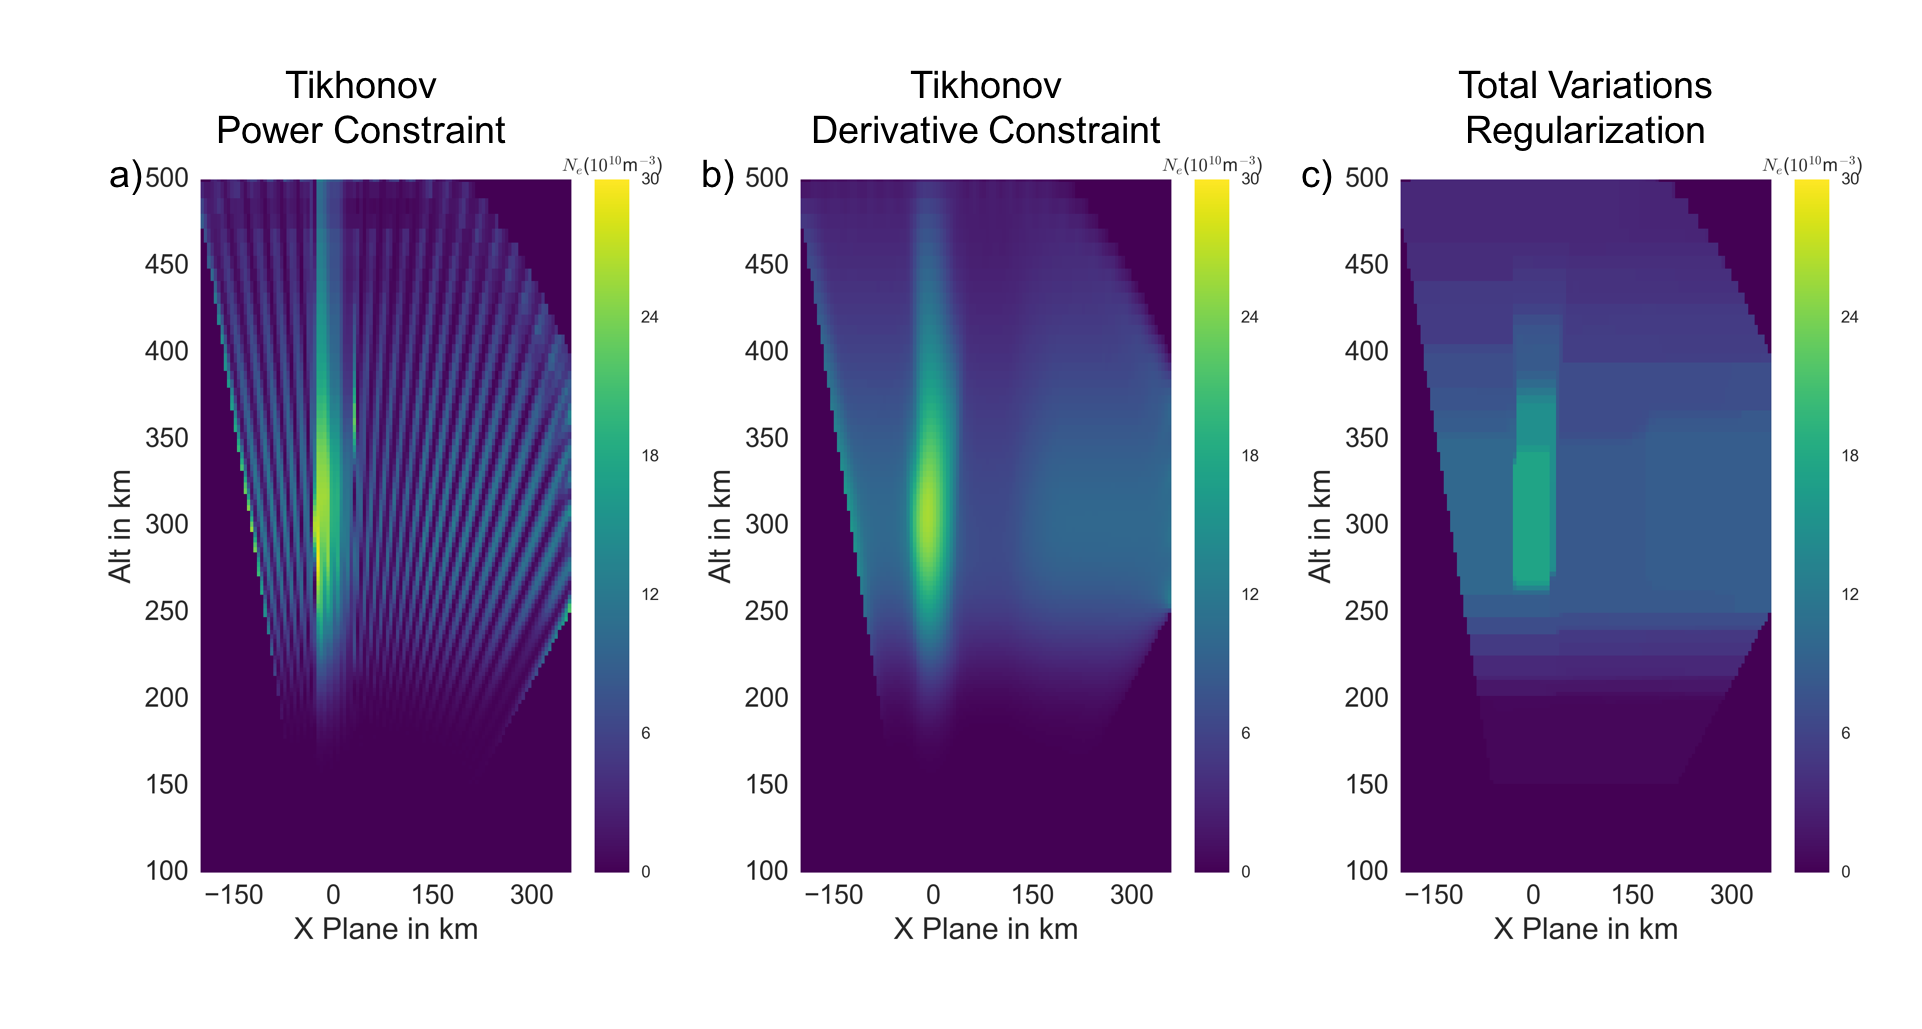
\includegraphics[width=6in]{Simpleinvertedfaster}
\caption{Results using the data in Figure~\ref{fig:simpinputfast}c to reconstruct the the $0^{th}$ lag: a) Using Equation \ref{eqn:tikpow}, Tikhonov constraint on $\mathbf{x}_{m,l}$.  b) Using Equation \ref{eqn:tikD}, Tikhonov constraint on $\mathbf{Dx}_{m,l}$. c) Using Equation \ref{eqn:tv}, Total Variations constraint.}
\label{fig:simpoutputfast}
\end{figure}

\subsection{Full Fitting Example}

In order to test the the results of the inversion method, a set of plasma parameters are used from \citet{Perry:2015jf} which show an auroral arc moving through the field of view at 200 m/s. The background plasma parameter values can be seen in Figure \ref{fig:plparamst0inv}. The field aligned current (FAC), which drives the arc, creates enhancements in electron density, electron and ion temperature. Also of importance is the plasma cavity which is co-located with the ion temperature enhancement and slightly ahead of the electron density enhancement. Perturbation features can be seen in Figure \ref{fig:plparamst960inv}, and using the same parameters 45 seconds later as the arc travels through the field of view yields Figure \ref{fig:plparamst1005inv}.

\begin{figure}[!ht]
\centering
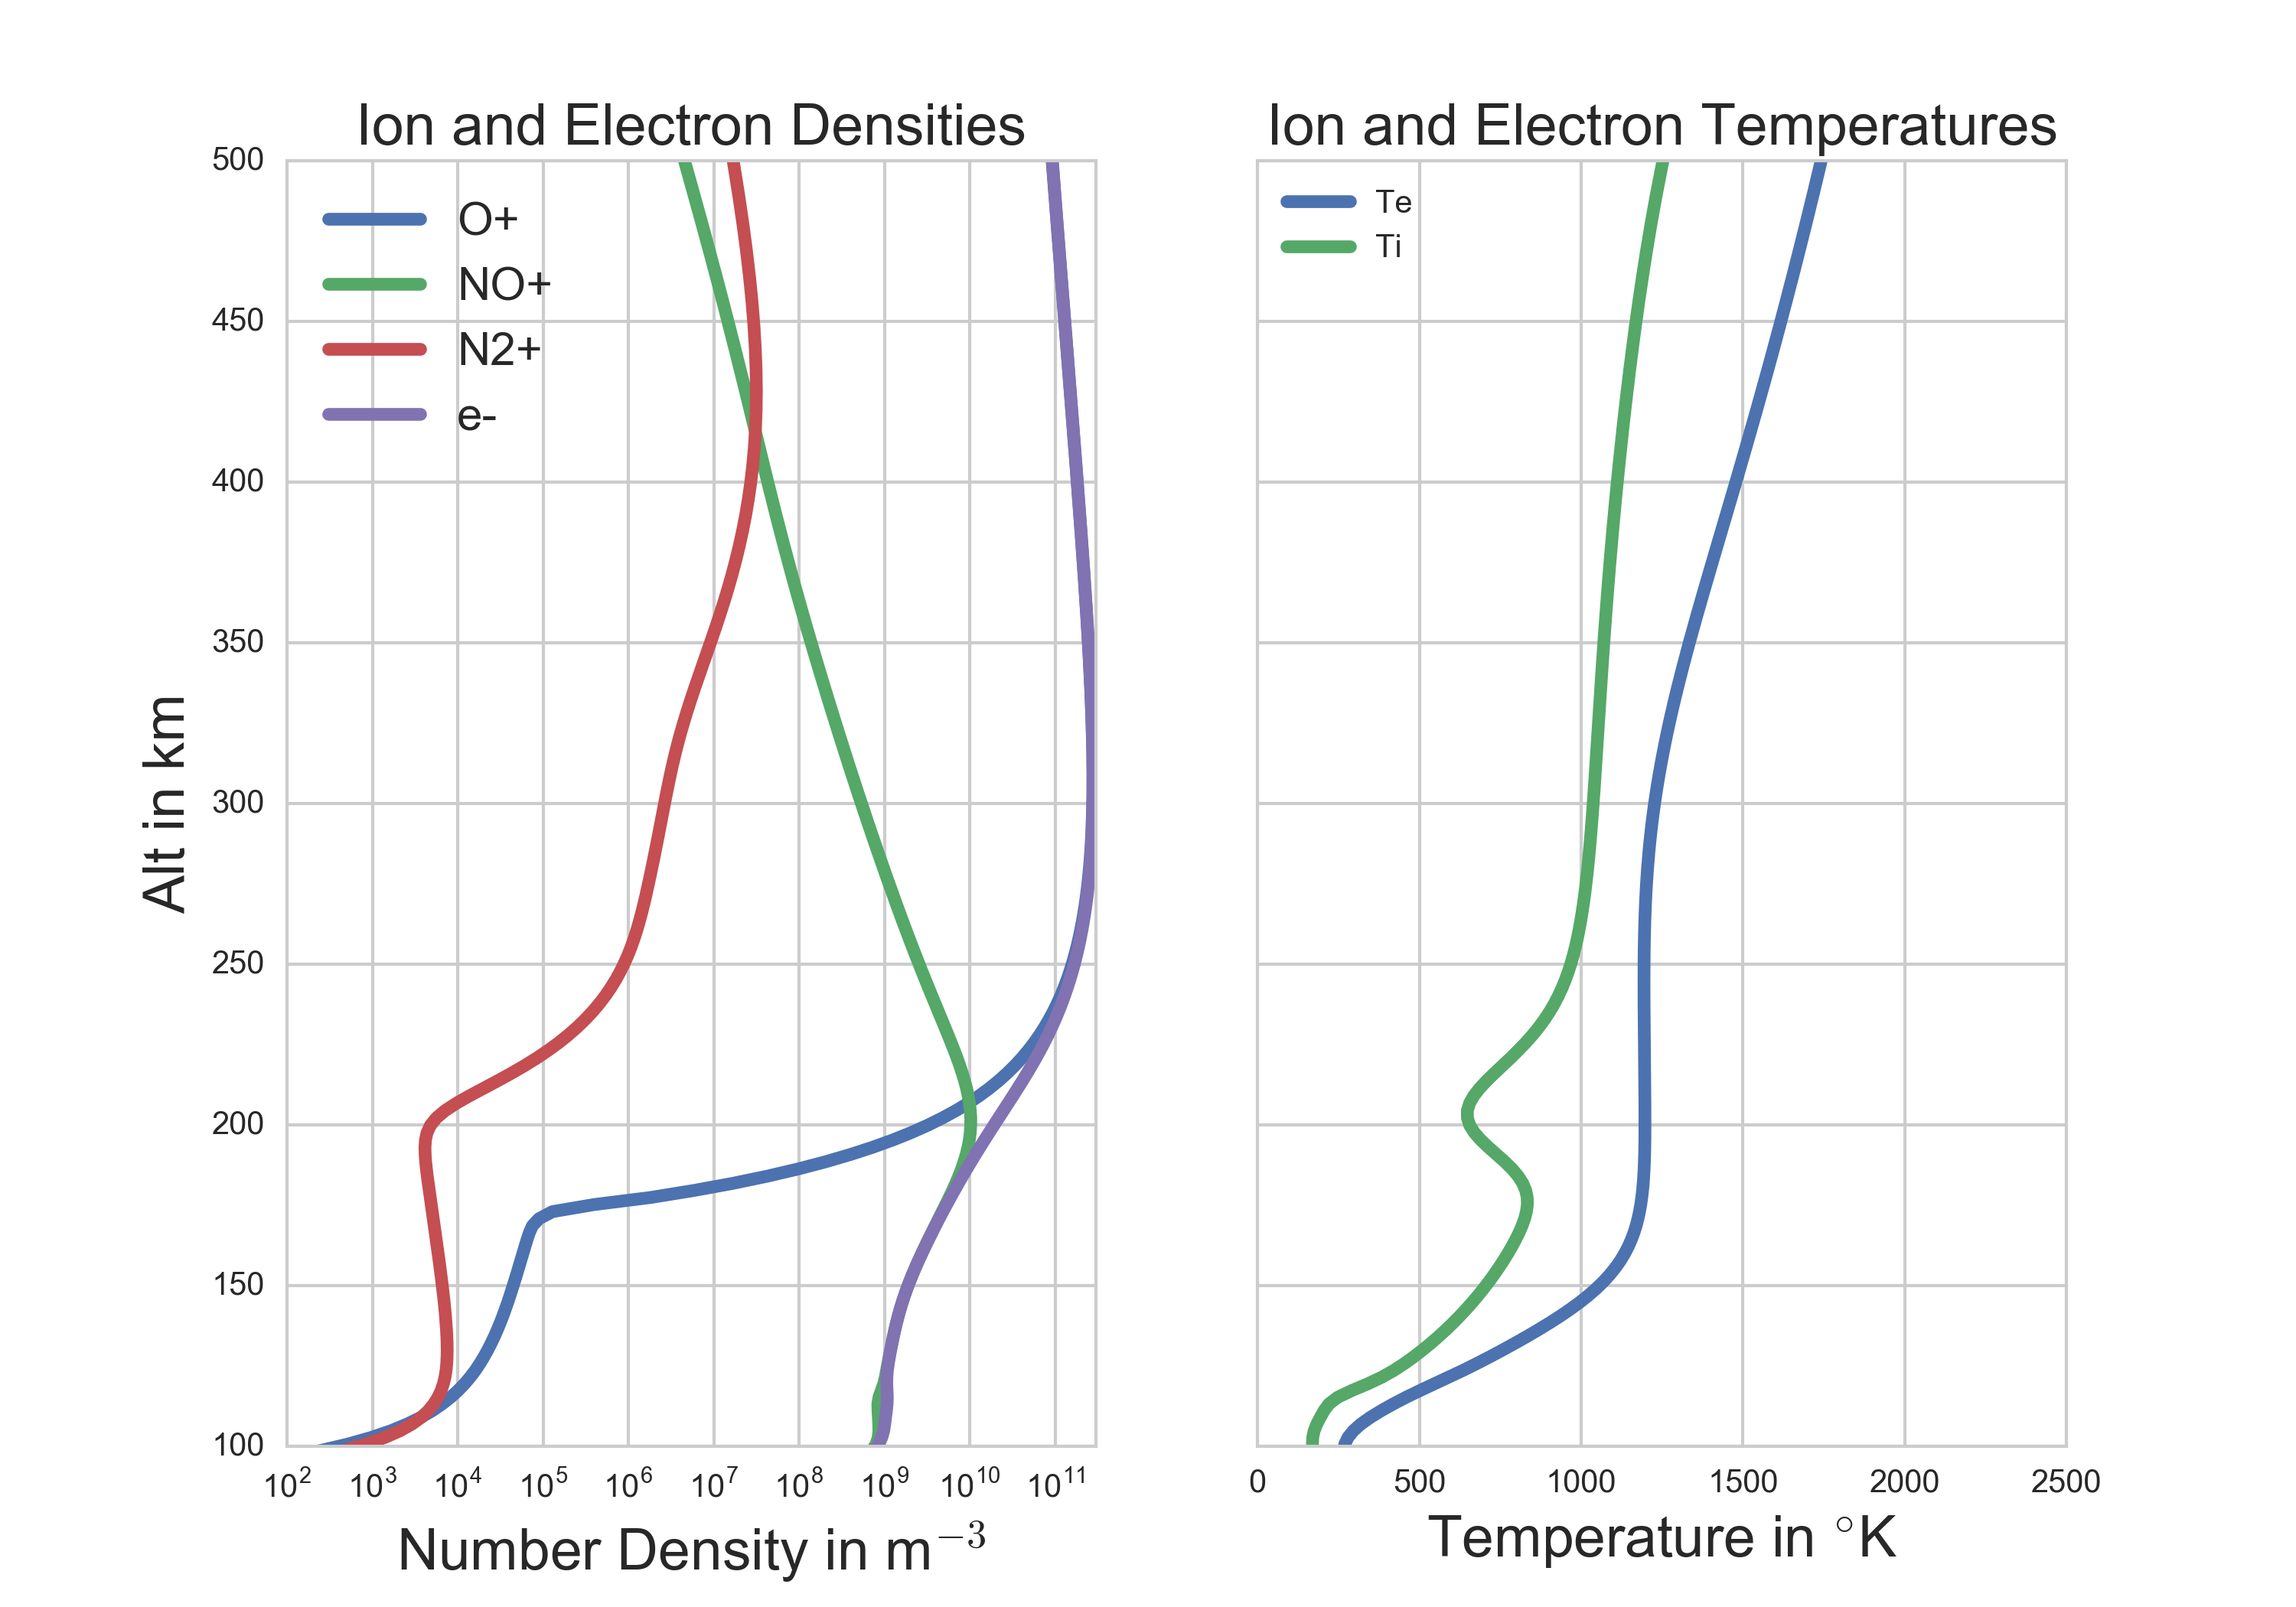
\includegraphics[width=6in]{backgroundallparams}
\caption{Background ionospheric parameters ($N_e$, $T_e$, $T_i$) along with number density of ion species, used for simulations.}
\label{fig:plparamst0inv}
\end{figure}

\begin{figure}[!ht]
\centering
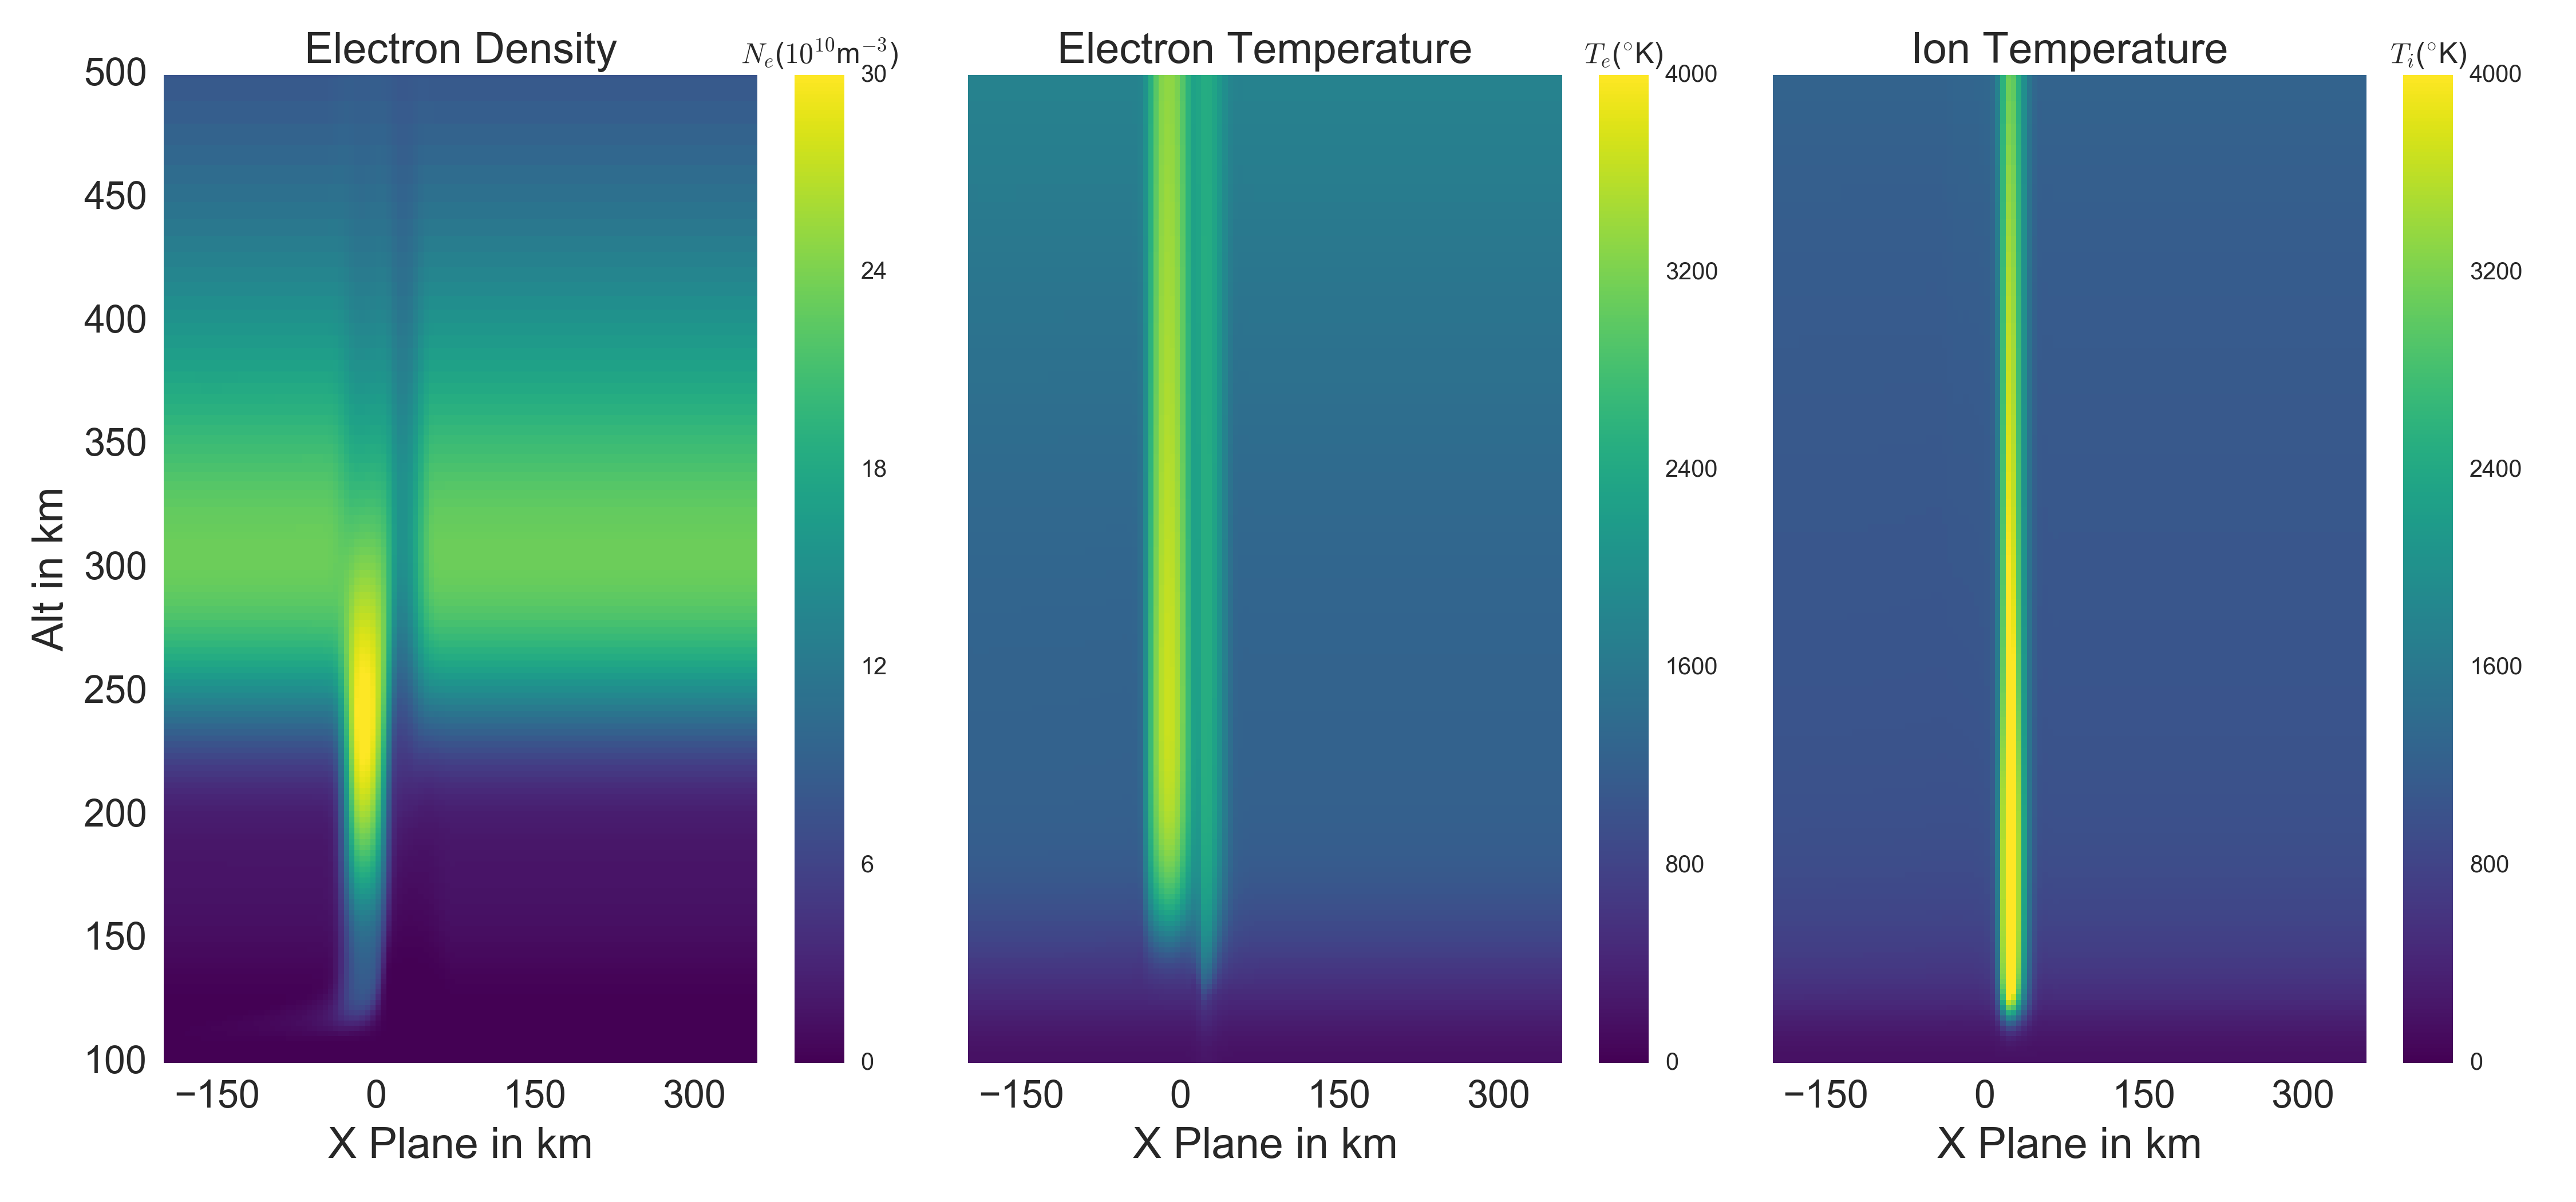
\includegraphics[width=6in]{0960_15_int}
\caption{Perturbations to Figure \ref{fig:plparamst0inv} due to an imposed current system of .875 $\mu$A/m$^2$ at $t=960$ s, auroral arc.}
\label{fig:plparamst960inv}
\end{figure}


\begin{figure}[!ht]
\centering
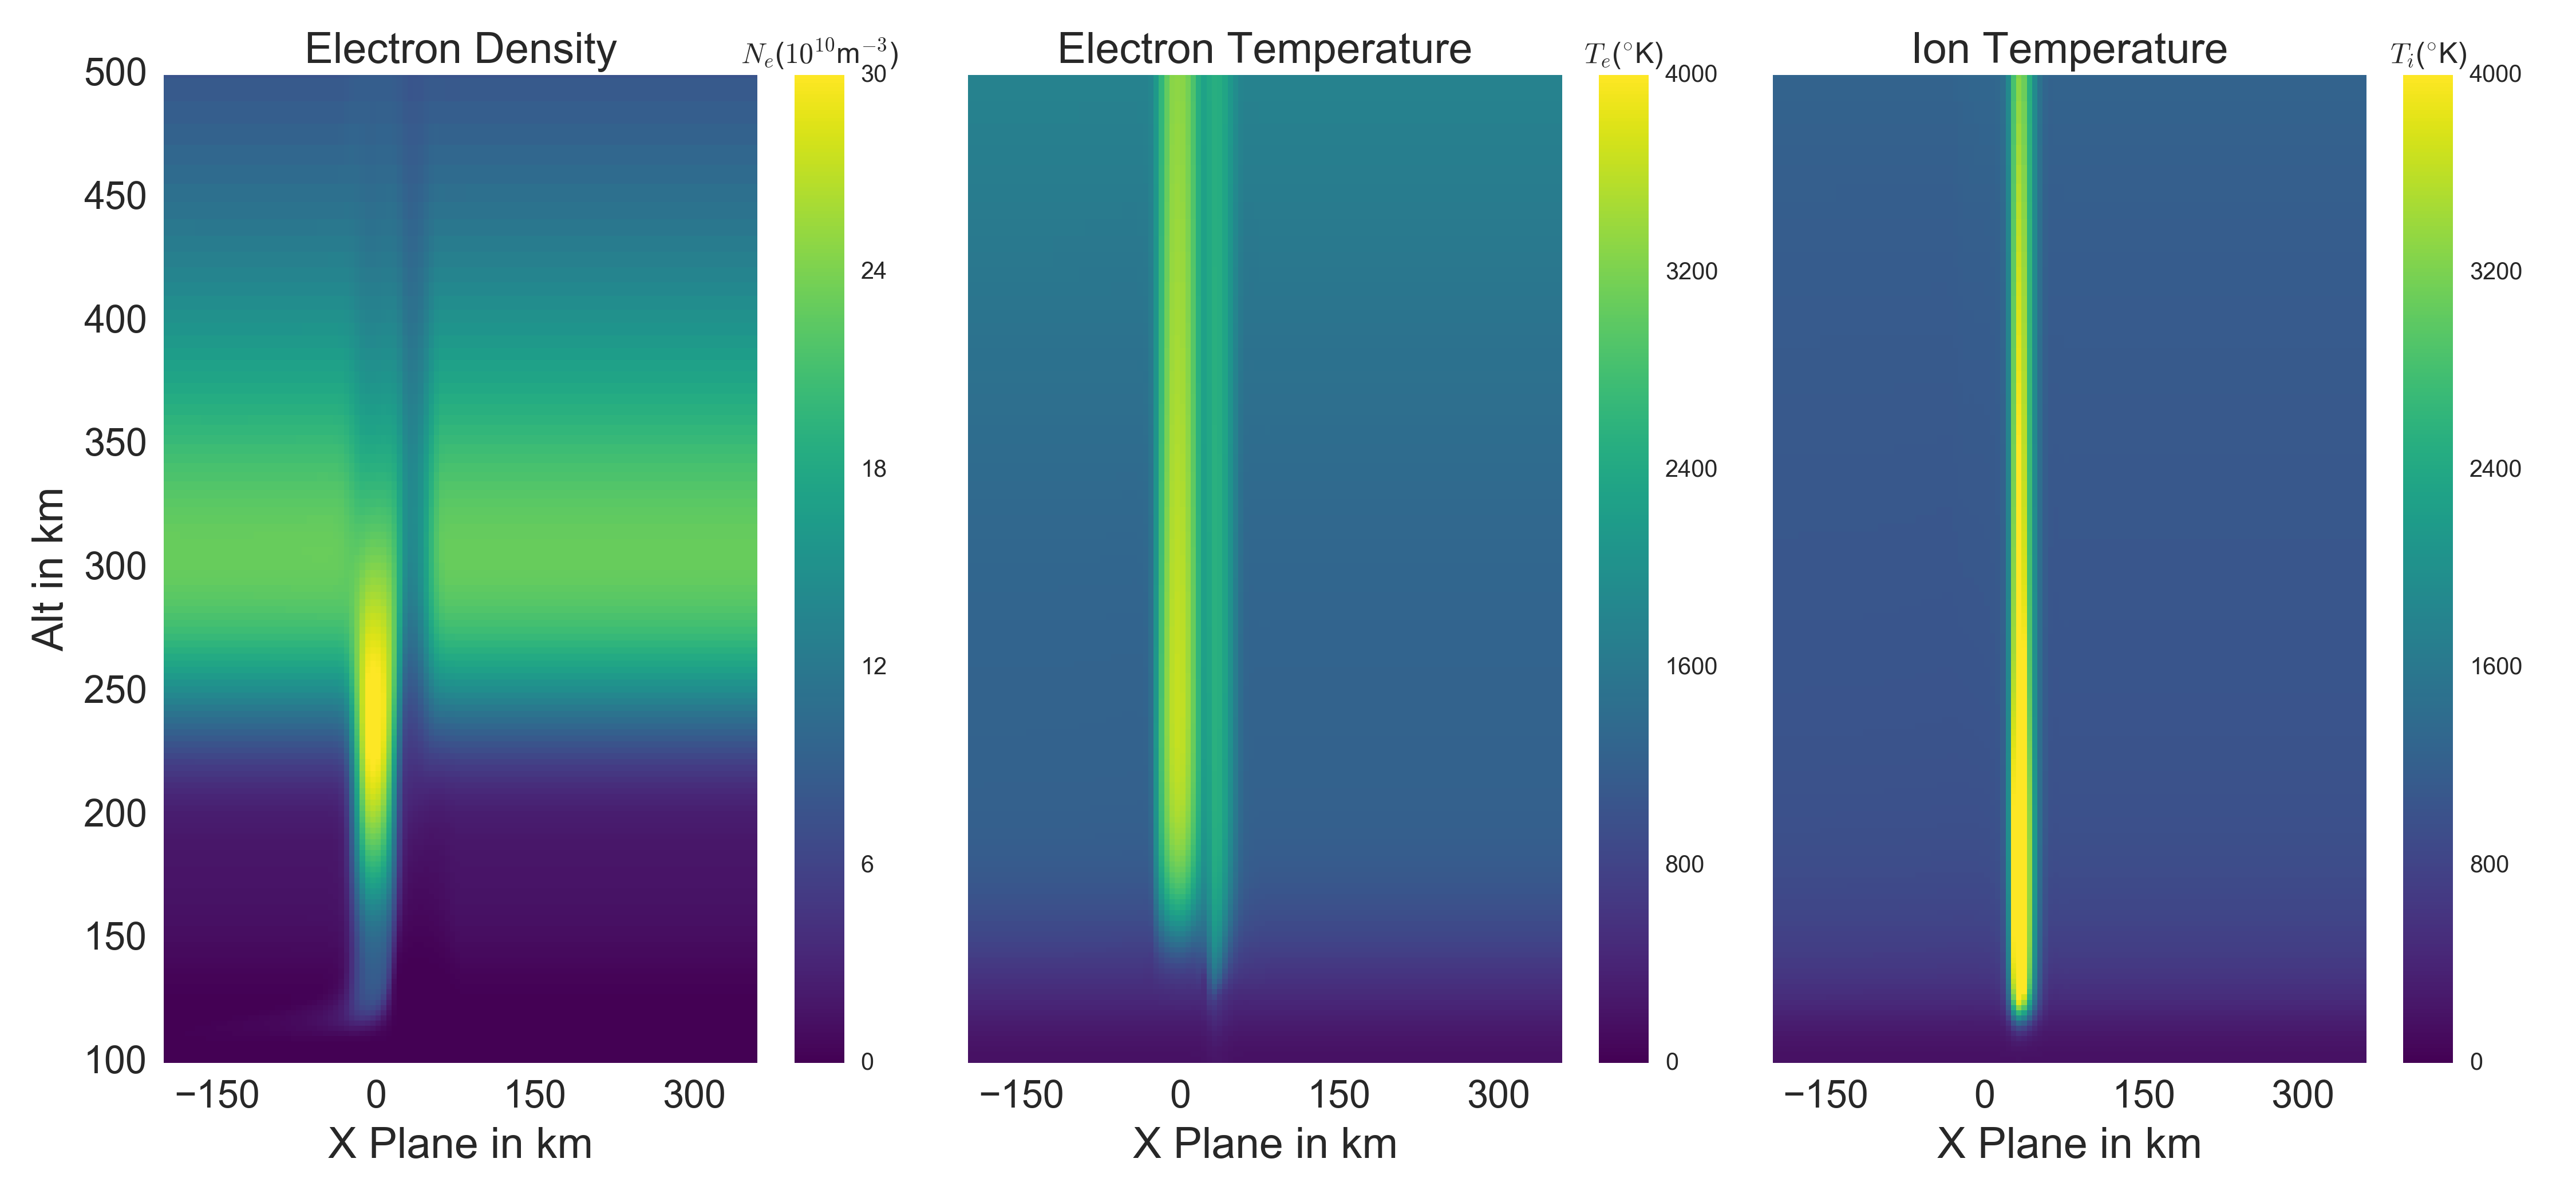
\includegraphics[width=6in]{1005_15_int}
\caption{Perturbations to Figure \ref{fig:plparamst0inv} due to an imposed current system of .875 $\mu$A/m$^2$ at $t=1005$ s, auroral arc.}
\label{fig:plparamst1005inv}
\end{figure}

The results using standard fitting, and then linearly interpolating the results, can be seen in Figure \ref{fig:fplparamst60inv} with associated expected errors in Figure \ref{fig:fplparamst60errinv}. The enhancements in $T_i$ and $T_e$ are visible although noisy. Also the depletion in $N_e$ is visible although this can be tied to the geometry of the beam pattern. The values seen in these patterns are also much larger then most of the errors seen in Figure \ref{fig:fplparamst60errinv} so there is some confidence in these fits.

% fitted data no inversion
\begin{figure}[!ht]
\centering
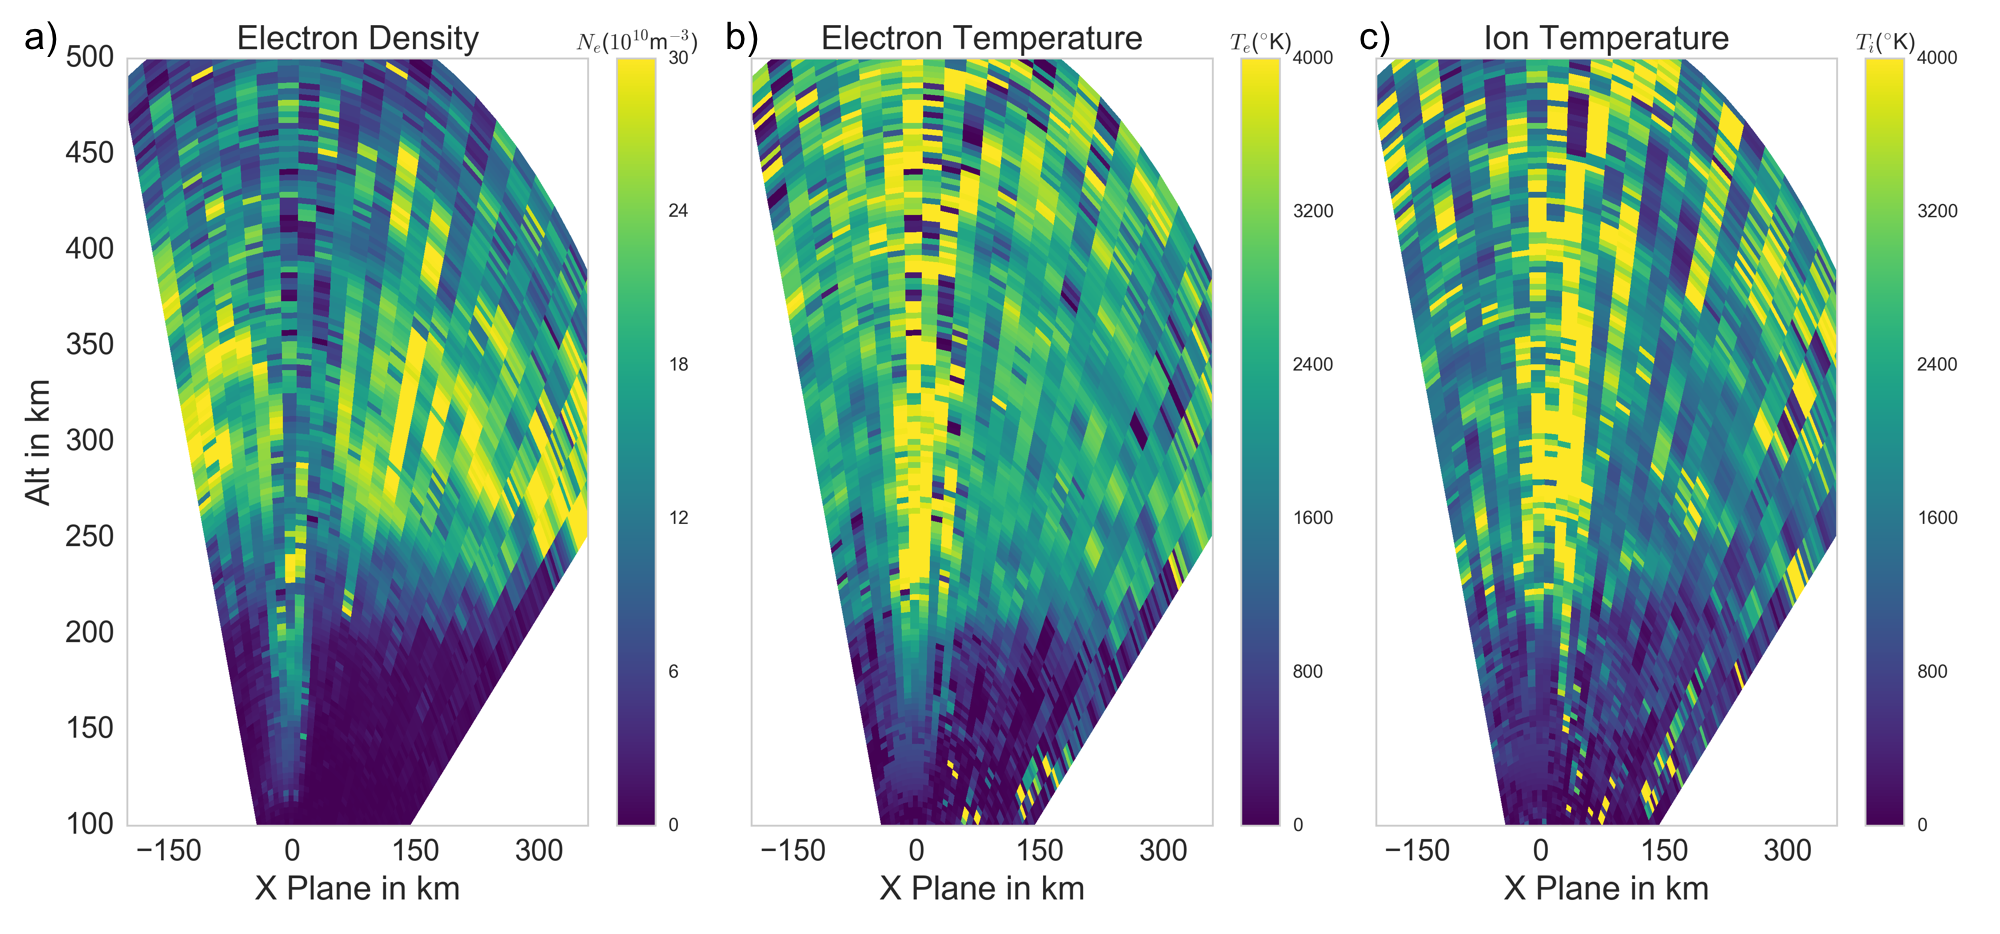
\includegraphics[width=6in]{0960_60_int}
\caption{Fitted Plasma Parameters at $t=960$ s with 60 second integration.}
\label{fig:fplparamst60inv}
\end{figure}

\begin{figure}[!ht]
\centering
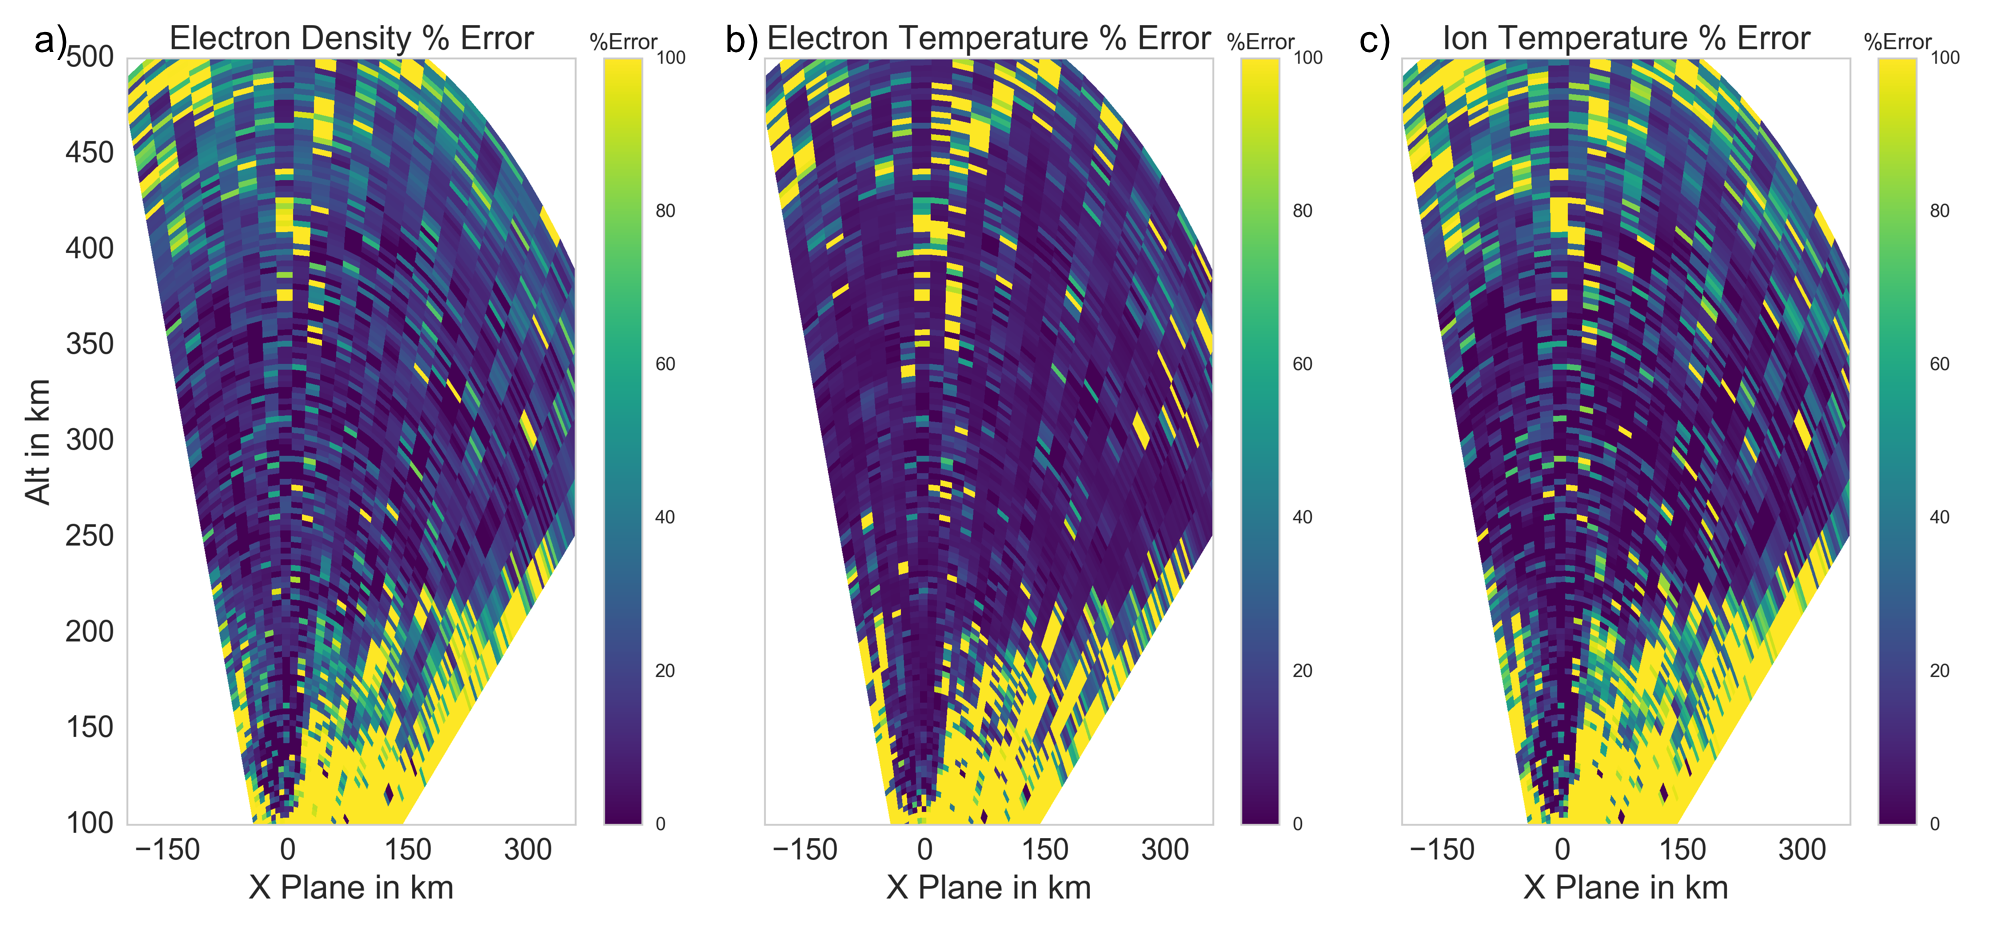
\includegraphics[width=6in]{0960_60_int_err}
\caption{Estimated errors from fitted Plasma Parameters at $t=960$ s with 60 second integration.}
\label{fig:fplparamst60errinv}
\end{figure}

% inverted and fitted data
The results of using the inversion algorithms can be seen in Figure \ref{fig:tikpow}, Figure \ref{fig:tikD} and Figure \ref{fig:tv}. The value for the $\gamma$ term for each type of inversion the algorithm is chosen by running the algorithms and taking the value that yields lowest mean squared error between the inverted lag and the original input ACF as in the previous section. 

The case using Tikhonov regularization where the $l^2$-norm of $\mathbf{x}_{m,l}$ is constrained is shown in Figure \ref{fig:tikpow}. An example ACF comparing the reconstruction to the input ACF and the estimated ACF using standard processing is shown in Figure \ref{fig:tikpowacf}. This specific case shows an inability of the constraint to fill in data that may be lost due to the specific beam position. This can also be seen in the ACF example as this reduced the amplitude of the ACF.

\begin{figure}[!ht]
\centering
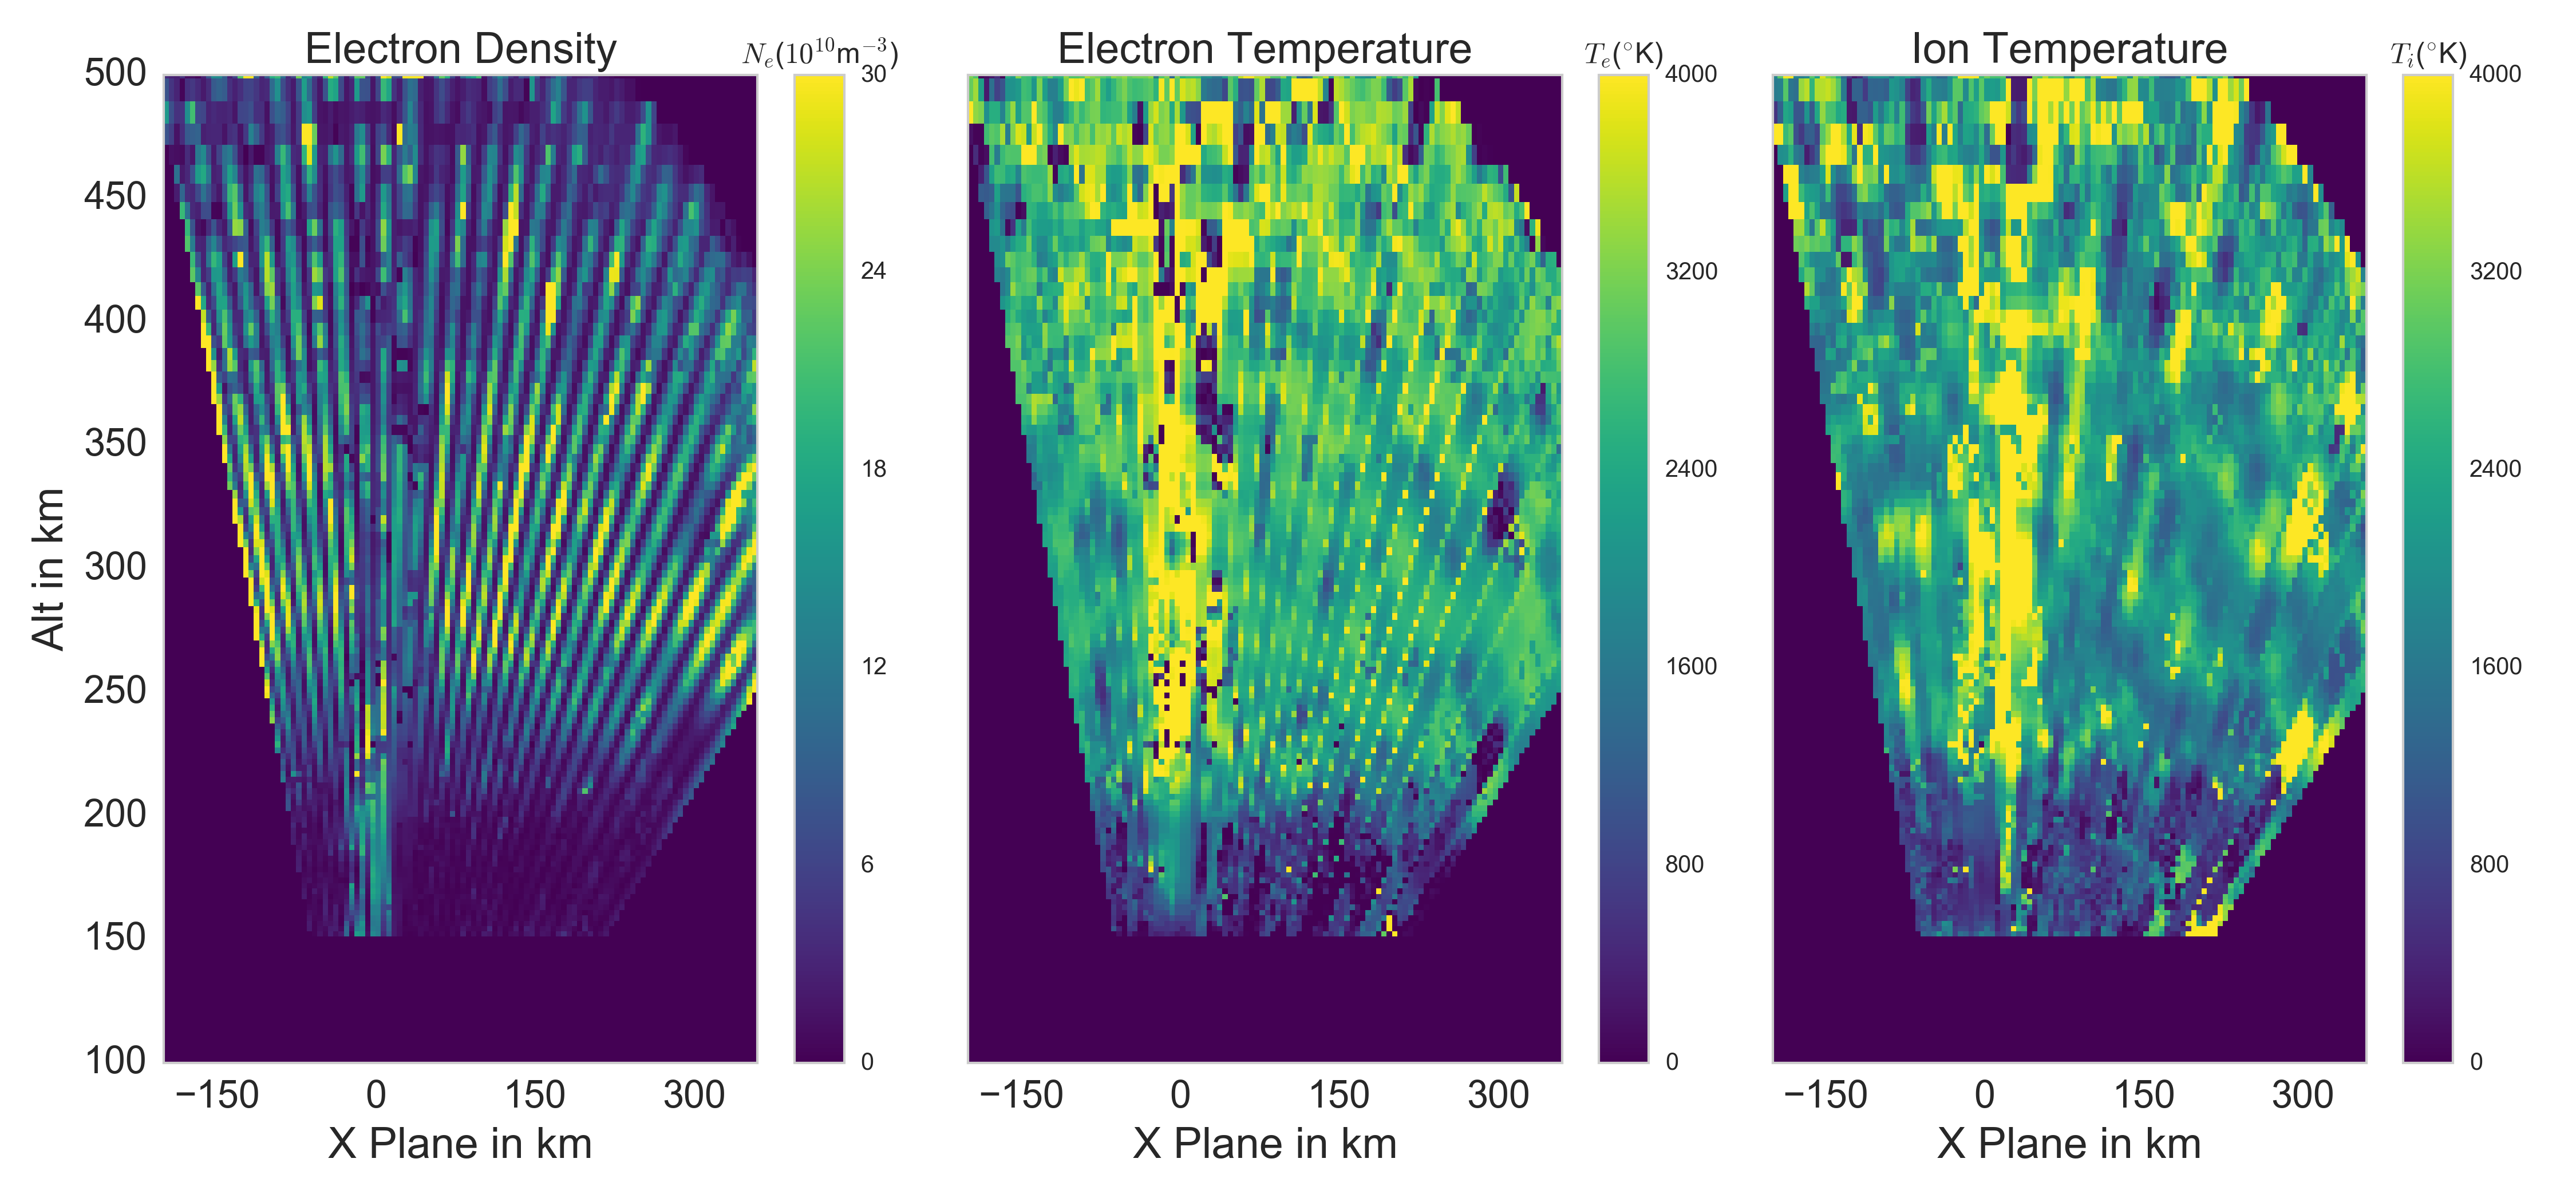
\includegraphics[width=6in]{tikfitted}
\caption{Fitted Plasma Parameters at $t=960$ s inverting lags with Equation \ref{eqn:tikpow}, Tikhonov constraint on $\mathbf{x}_{m,l}$. }
\label{fig:tikpow}
\end{figure}

\begin{figure}[!ht]
\centering
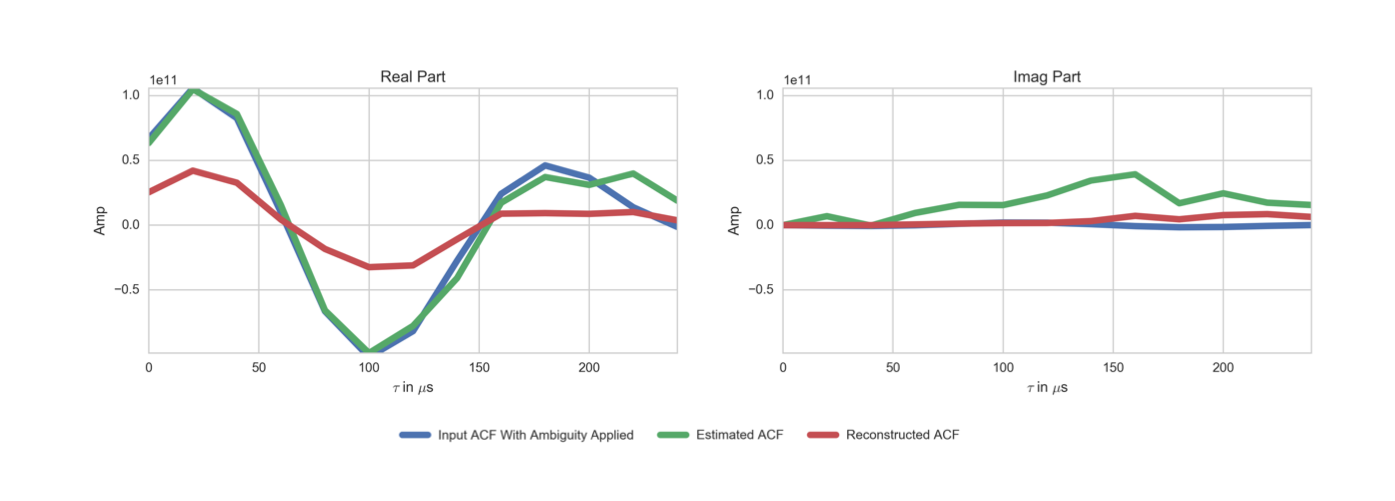
\includegraphics[width=6in]{acftik}
\caption{Example ACF at time $t=960$ s and location $\mathbf{r}=[0  \text{ km}, 250 \text{ km}]^T$ with reconstructing lags using Equation \ref{eqn:tikpow}, Tikhonov constraint on $\mathbf{x}_{m,l}$. }
\label{fig:tikpowacf}
\end{figure}

The image in Figure \ref{fig:tikD} is the result of using Tikhonov regularization on the spatial gradient of each lag of the ACF. This leads to an apparent smoothing of the plasma parameters but many of the important features in this simulation, such as the depletion in $N_e$ and enhancements in $T_e$ and $T_i$ are visible and more obvious than in Figure \ref{fig:fplparamst60inv}. An example ACF comparing the reconstruction to the input ACF and the estimated ACF using standard processing is shown in Figure \ref{fig:tikDacf}. The example reconstructed ACF does show more deviations from the input in the real part but at the higher lags it more closely resembles the true ACF. The imaginary part though, is much closer to the real ACF as this possibly reduced and random Doppler shifts.
\begin{figure}[!ht]
\centering
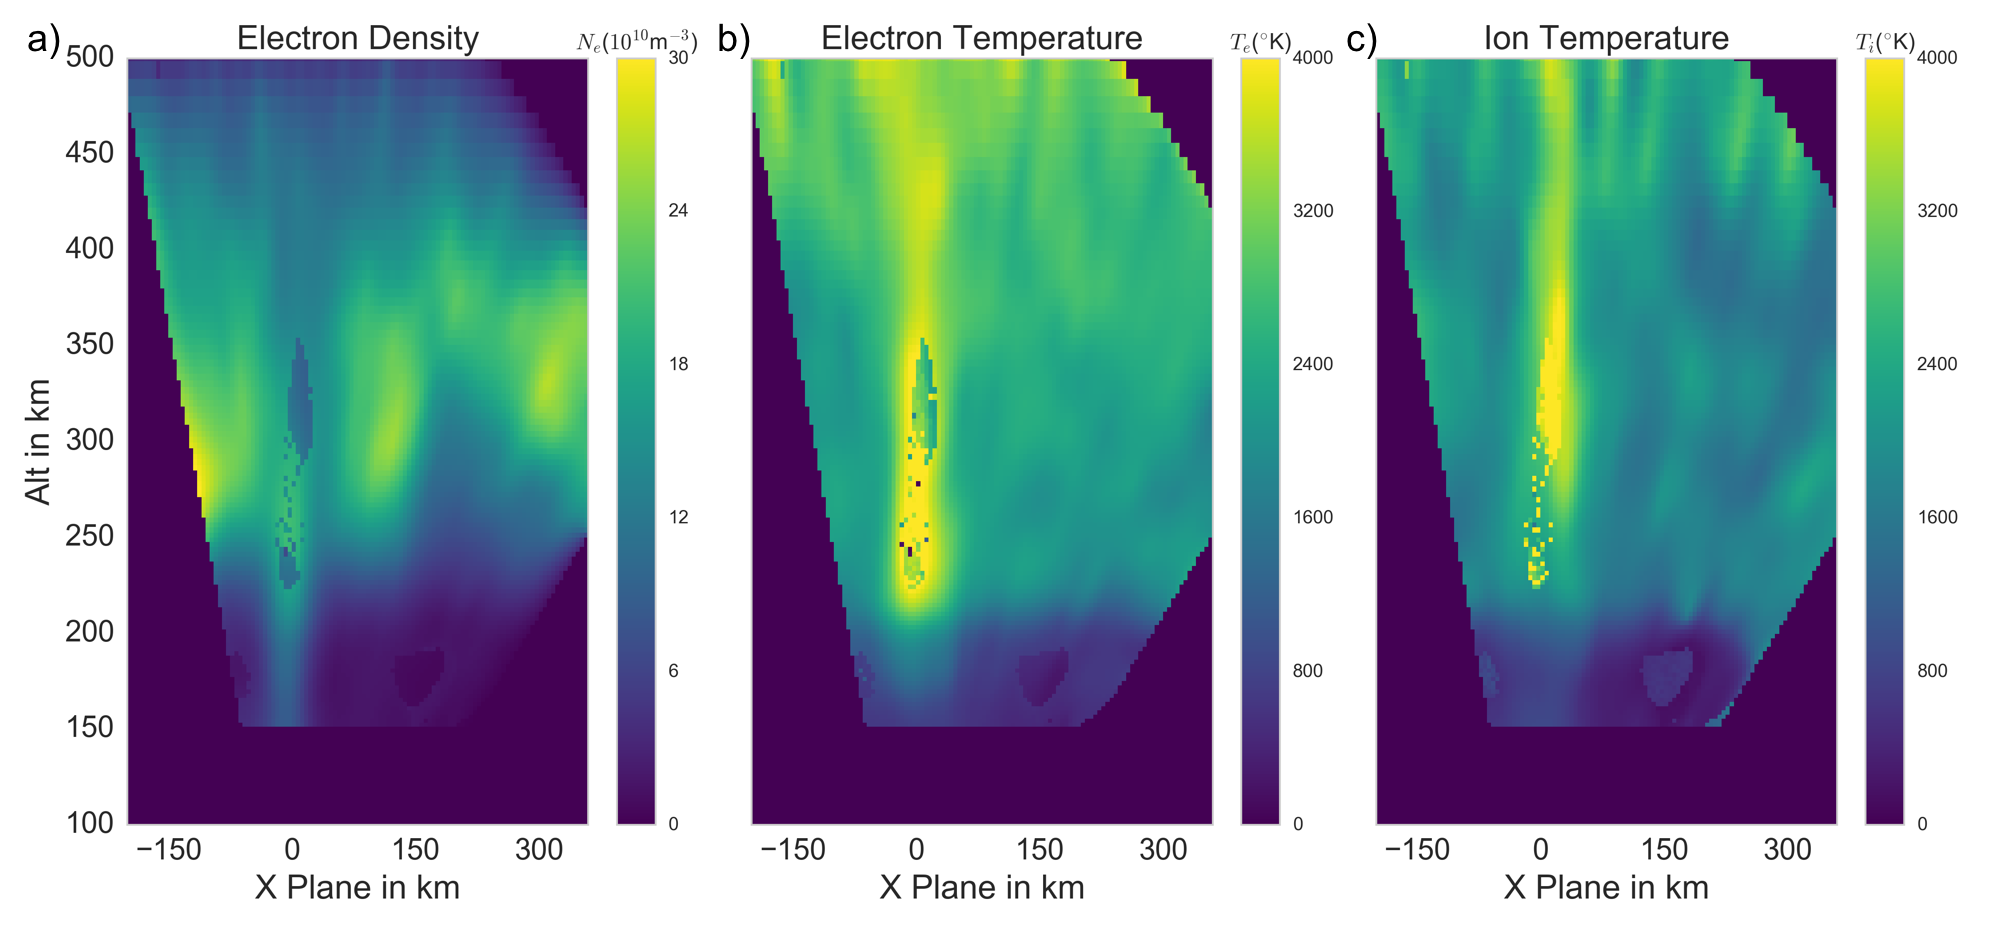
\includegraphics[width=6in]{tikdfitted}
\caption{Fitted Plasma Parameters at $t=960$ s inverting lags with Equation \ref{eqn:tikD}, Tikhonov constraint on $\mathbf{Dx}_{m,l}$. }
\label{fig:tikD}
\end{figure}

\begin{figure}[!ht]
\centering
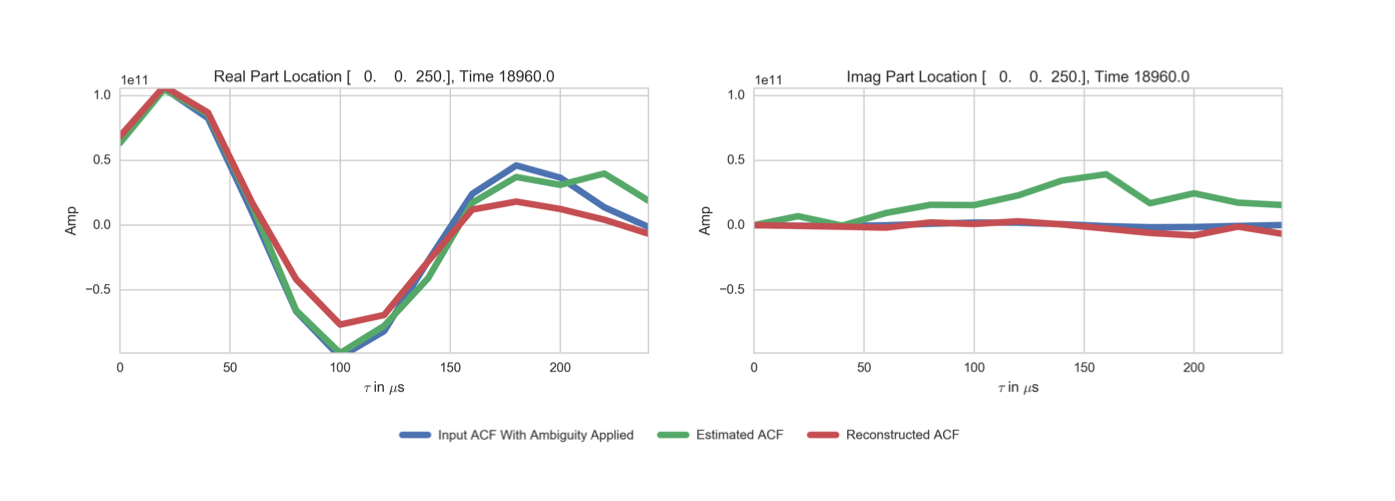
\includegraphics[width=6in]{acftikd}
\caption{Example ACF at time $t=960$ s and location $\mathbf{r}=[0  \text{ km}, 250 \text{ km}]^T$ with reconstructing lags using Equation \ref{eqn:tikpow}, Tikhonov constraint on $\mathbf{Dx}_{m,l}$. }
\label{fig:tikDacf}
\end{figure}

Lastly for this case the result of the inversion using the total variations constraint is shown in Figure \ref{fig:tv}. This inversion method shows the features discussed earlier but they take on a``blocky" look, as was seen in the zeroth lag case. An example ACF comparing the reconstruction to the input ACF and the estimated ACF using standard processing is shown in Figure \ref{fig:tvacf}. This shows similar behavior to the reconstruction ACF in Figure \ref{fig:tikDacf}, although the imaginary part of the ACF is much closer to the true value of zero.
\begin{figure}[!ht]
\centering
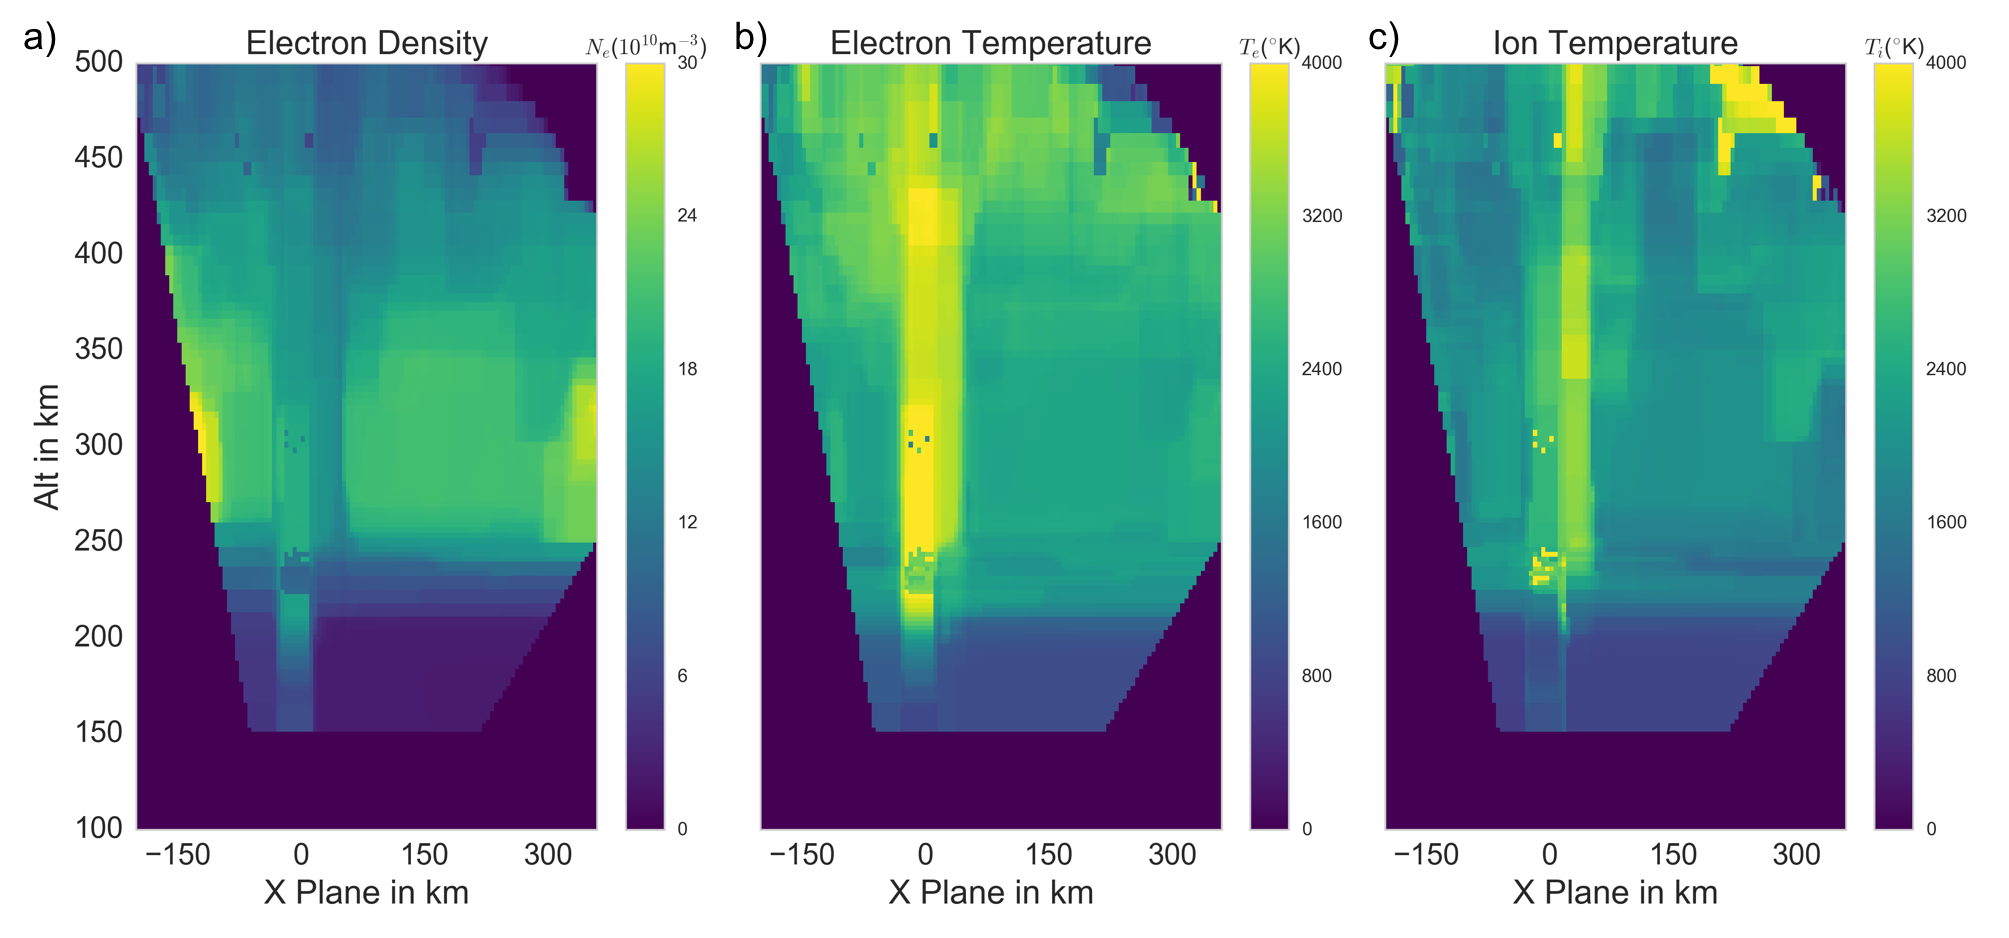
\includegraphics[width=6in]{tvfitted}
\caption{Fitted Plasma Parameters at $t=960$ s inverting lags with Equation \ref{eqn:tv}, Total Variations constraint.}
\label{fig:tv}
\end{figure}

\begin{figure}[!ht]
\centering
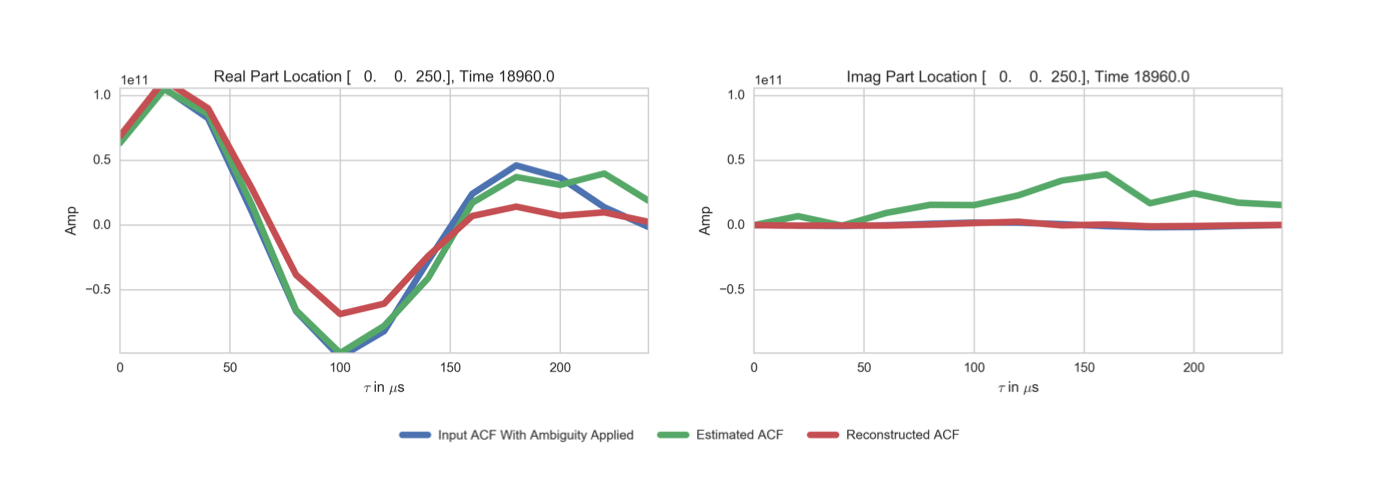
\includegraphics[width=6in]{acftv}
\caption{Example ACF at time $t=960$ s and location$\mathbf{r}=[0  \text{ km}, 250 \text{ km}]^T$ reconstructing lags using Equation \ref{eqn:tv}, Total Variations constraint. }
\label{fig:tvacf}
\end{figure}

\section{Summary}

This chapter has discussed a method for reconstructing plasma parameters from ESA ISR measurements in the frame of reference of the moving plasma. The space-time ambiguity, described in Chapter 3, straightforwardly allows for this. Currently a number of simplifying assumptions are made to get a basic reconstruction. The initial results are promising although more work needs to be done to improve this method and determine its limits as more and more realistic aspects are added.